%%%%%%%%%%%%%%%%%%%%%%%%%%%%%%%%%%%%%%%%%%%%%%%%%%%%%%%%%%%%%%%%%%%%%%%%%%%%%%%%%%%%%%%%%%%%%%%%%%%%%%%%%%%%%%%%%%%%%%%%%%%%%%%%%%%%%%%%%%%%%%%%%%%%%%%%%%%
% This is just an example/guide for you to refer to when producing your supplementary material for your Frontiers article.                                 %
%%%%%%%%%%%%%%%%%%%%%%%%%%%%%%%%%%%%%%%%%%%%%%%%%%%%%%%%%%%%%%%%%%%%%%%%%%%%%%%%%%%%%%%%%%%%%%%%%%%%%%%%%%%%%%%%%%%%%%%%%%%%%%%%%%%%%%%%%%%%%%%%%%%%%%%%%%%

%%% Version 2.5 Generated 2018/06/15 %%%
%%% You will need to have the following packages installed: datetime, fmtcount, etoolbox, fcprefix, which are normally inlcuded in WinEdt. %%%
%%% In http://www.ctan.org/ you can find the packages and how to install them, if necessary. %%%
%%%  NB logo1.jpg is required in the path in order to correctly compile front page header %%%

\documentclass[utf8]{frontiers_suppmat} % for all articles
\usepackage{url,hyperref,lineno,microtype}
\usepackage[onehalfspacing]{setspace}



% Leave a blank line between paragraphs instead of using \\

\begin{document}
\onecolumn
\firstpage{1}

\title[Supplementary Material]{{\helveticaitalic{Supplementary Material}}}


\maketitle

%%%%%%%%%%%%%%%%%%%%%%%%%%%%%%%%%%%%%%%%%%%%%%%%%%%%%%%%%%%%%%%%%%%%%%%%%%%%%
\section{Differences with Bianchi et al., 2017}
%%%%%%%%%%%%%%%%%%%%%%%%%%%%%%%%%%%%%%%%%%%%%%%%%%%%%%%%%%%%%%%%%%%%%%%%%%%%%

A part of this study does the same analysis as Bianchi et al., 2017.
mainly concern the use of different
software and a different definition of what an MHC binder is.

% \paragraph{Definition of what a binder is}

The earlier study defined a peptide an MHC binder 
if \emph{within the protein} in which it was found, 
is was among the peptides with the 2\% lowest IC50 values.
This can be seen at \url{https://github.com/richelbilderbeek/bianchi_et_al_2017/blob/master/predict-binders.R},
where the binders are written to file.

However, in this study, an MHC binder is defined as a peptide within a \emph{proteome} in which it is found, that is among the peptides with the 2\% lowest IC50 values.
Subsection \ref{subsec:ic50s_per_haplotype} shows the IC50 values
for a binder per MHC allele. 

% \paragraph{Selenoproteins}

Our previous study used the TMHMM web server
to predict TMHs.
The desktop version of TMHMM, however, gives an
error message on the 25 selenoproteins found in the human
reference proteome.
For the sake of reproducible research, we used the desktop version (as
we can call it from scripts) and, due to this, we removed the
selenoproteins from this analysis.

% \paragraph{Compare results in figure}

To verify if the previous and the current method give rise to
notable difference, we show a side-by-side comparison
in figures \ref{fig:bianch_et_al_2017_1a} and \ref{fig:bilderbeek_et_al_2021_1a}.
The figures that MHC molecules that over-present or under-present TMH-derived epitopes,
do so in both studies. The extent to which TMH-derived epitopes are
presented, however, is more extreme in our current setup.

\begin{figure}[h!]
\begin{center}
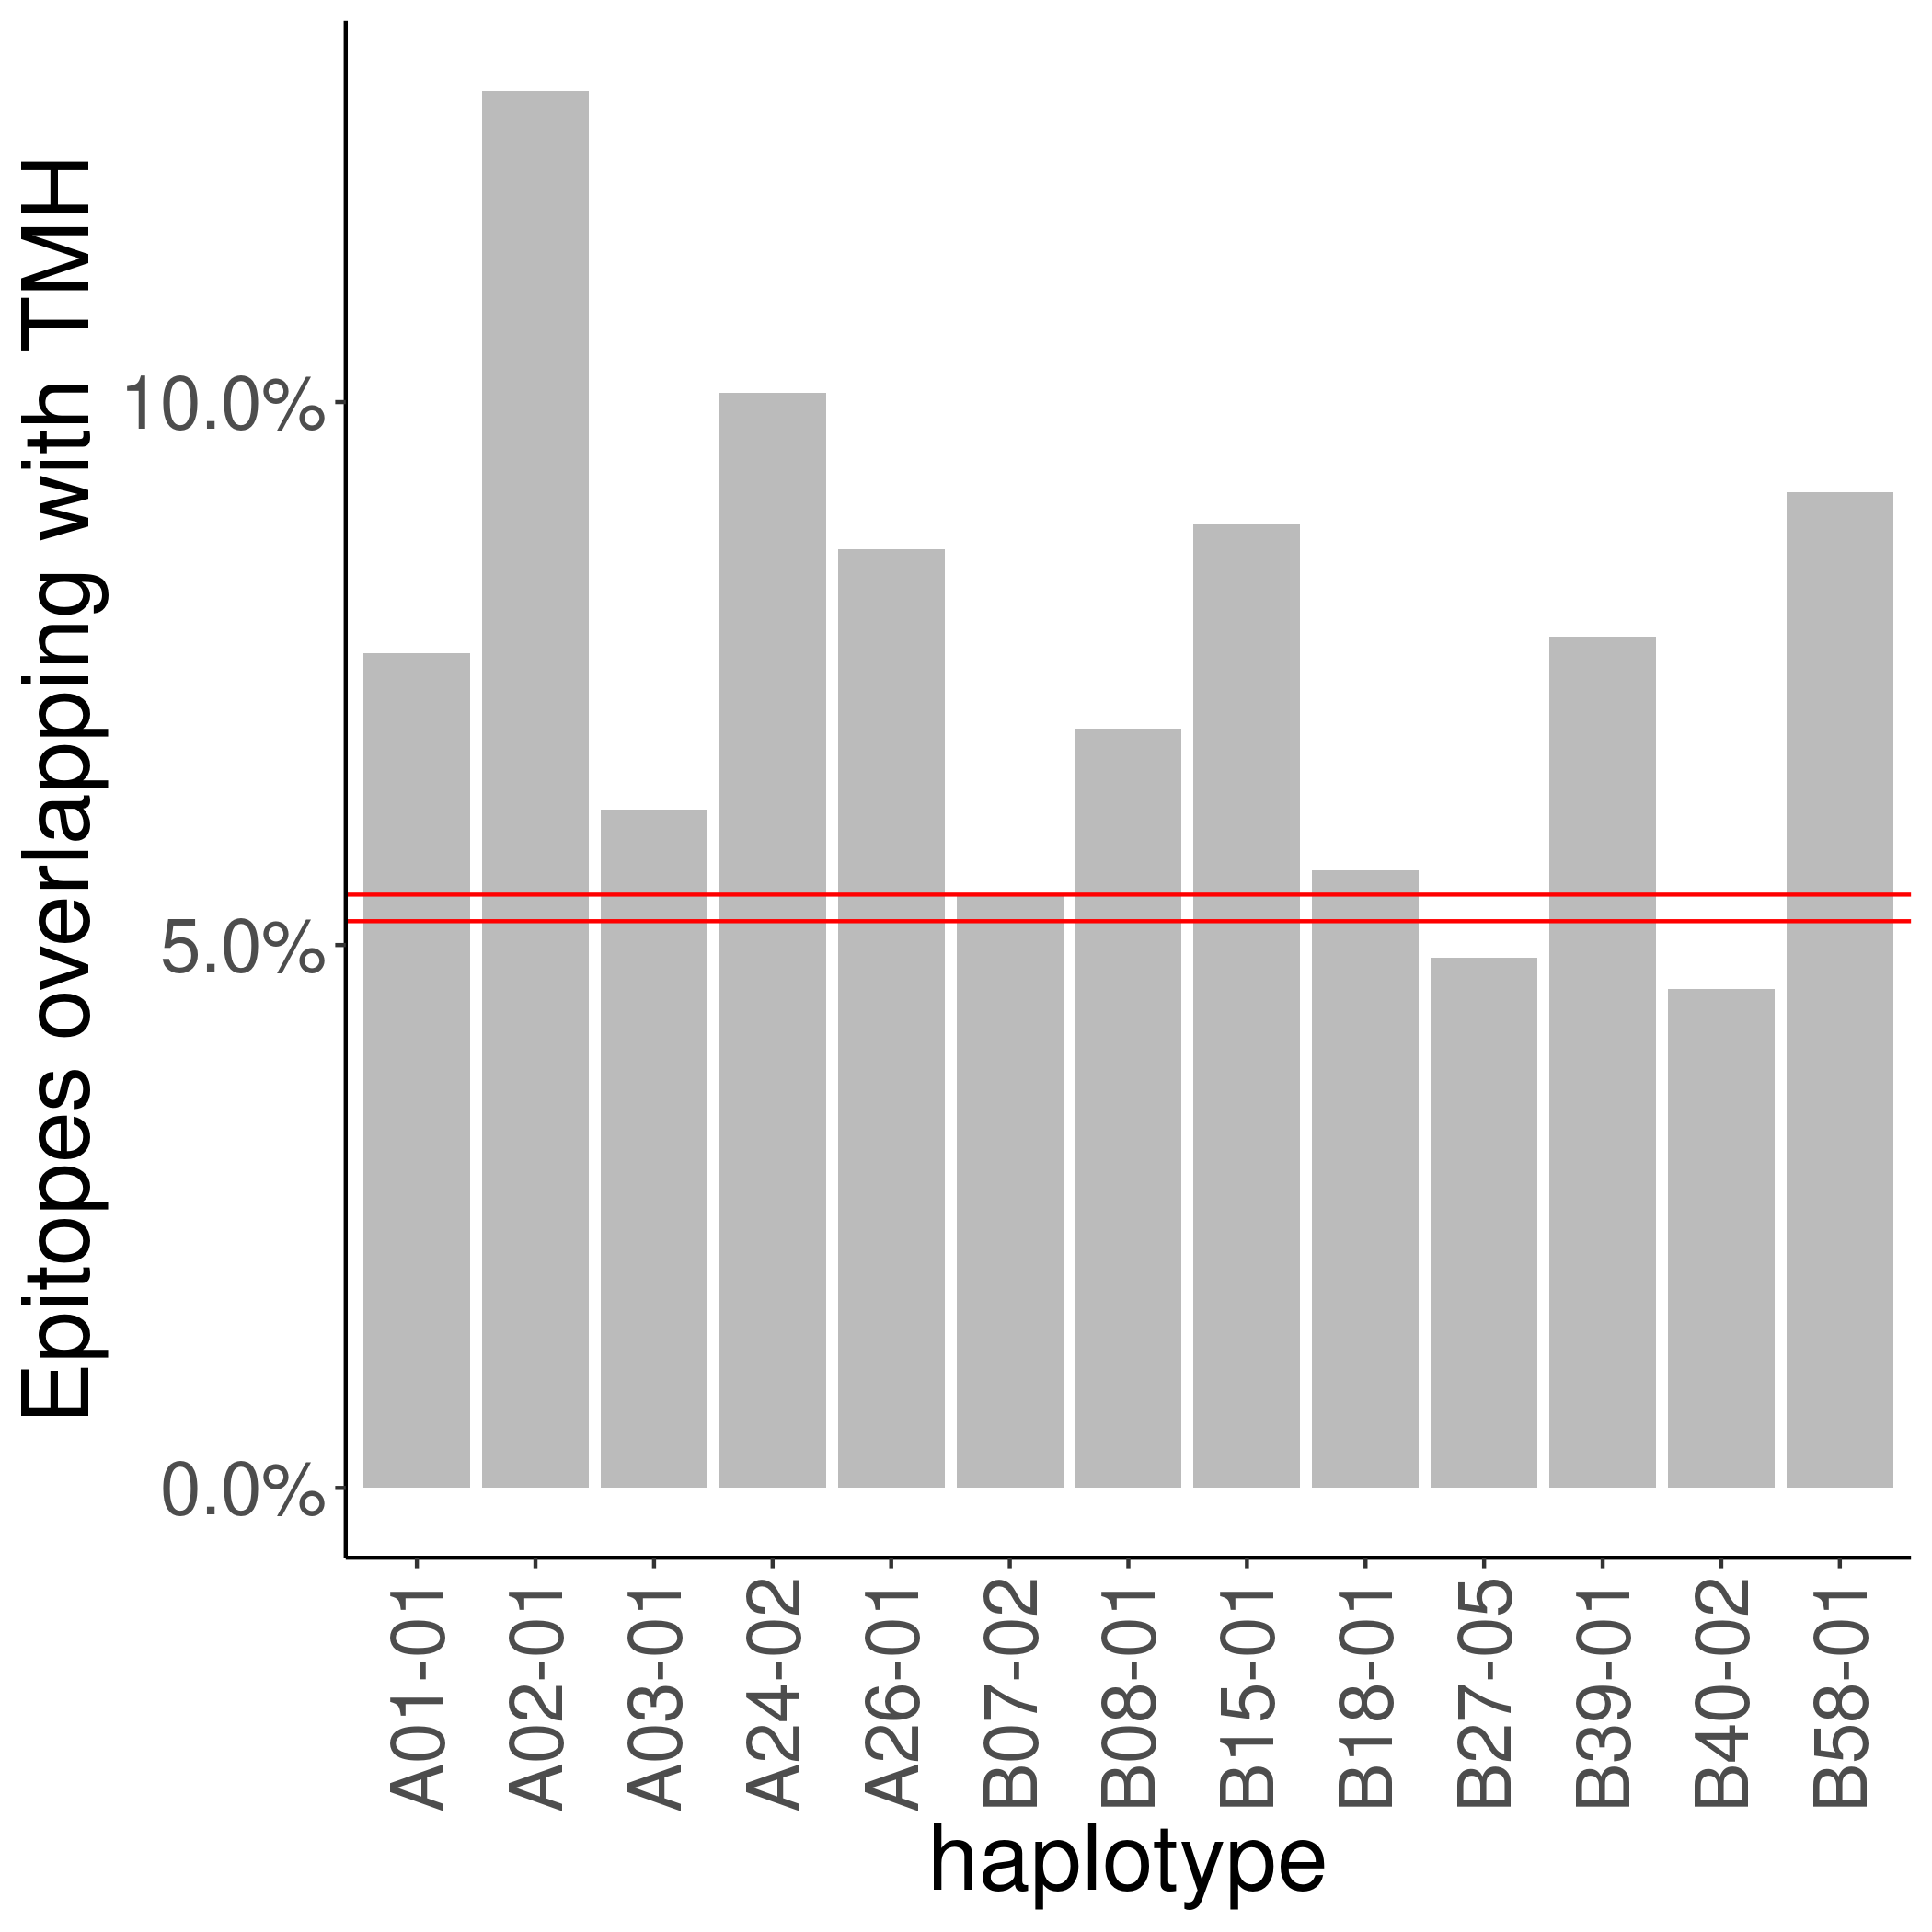
\includegraphics[width=\linewidth]{bianchi_et_al_2017_results/figure-1-a.png} % use same naming as them
\end{center}
\caption{
    Results for \citep{bianchi2017}. 
    Dashed lines denotes the coincidence interval.
}
\label{fig:bianch_et_al_2017_1a}
\end{figure}

\begin{figure}[h!]
\begin{center}
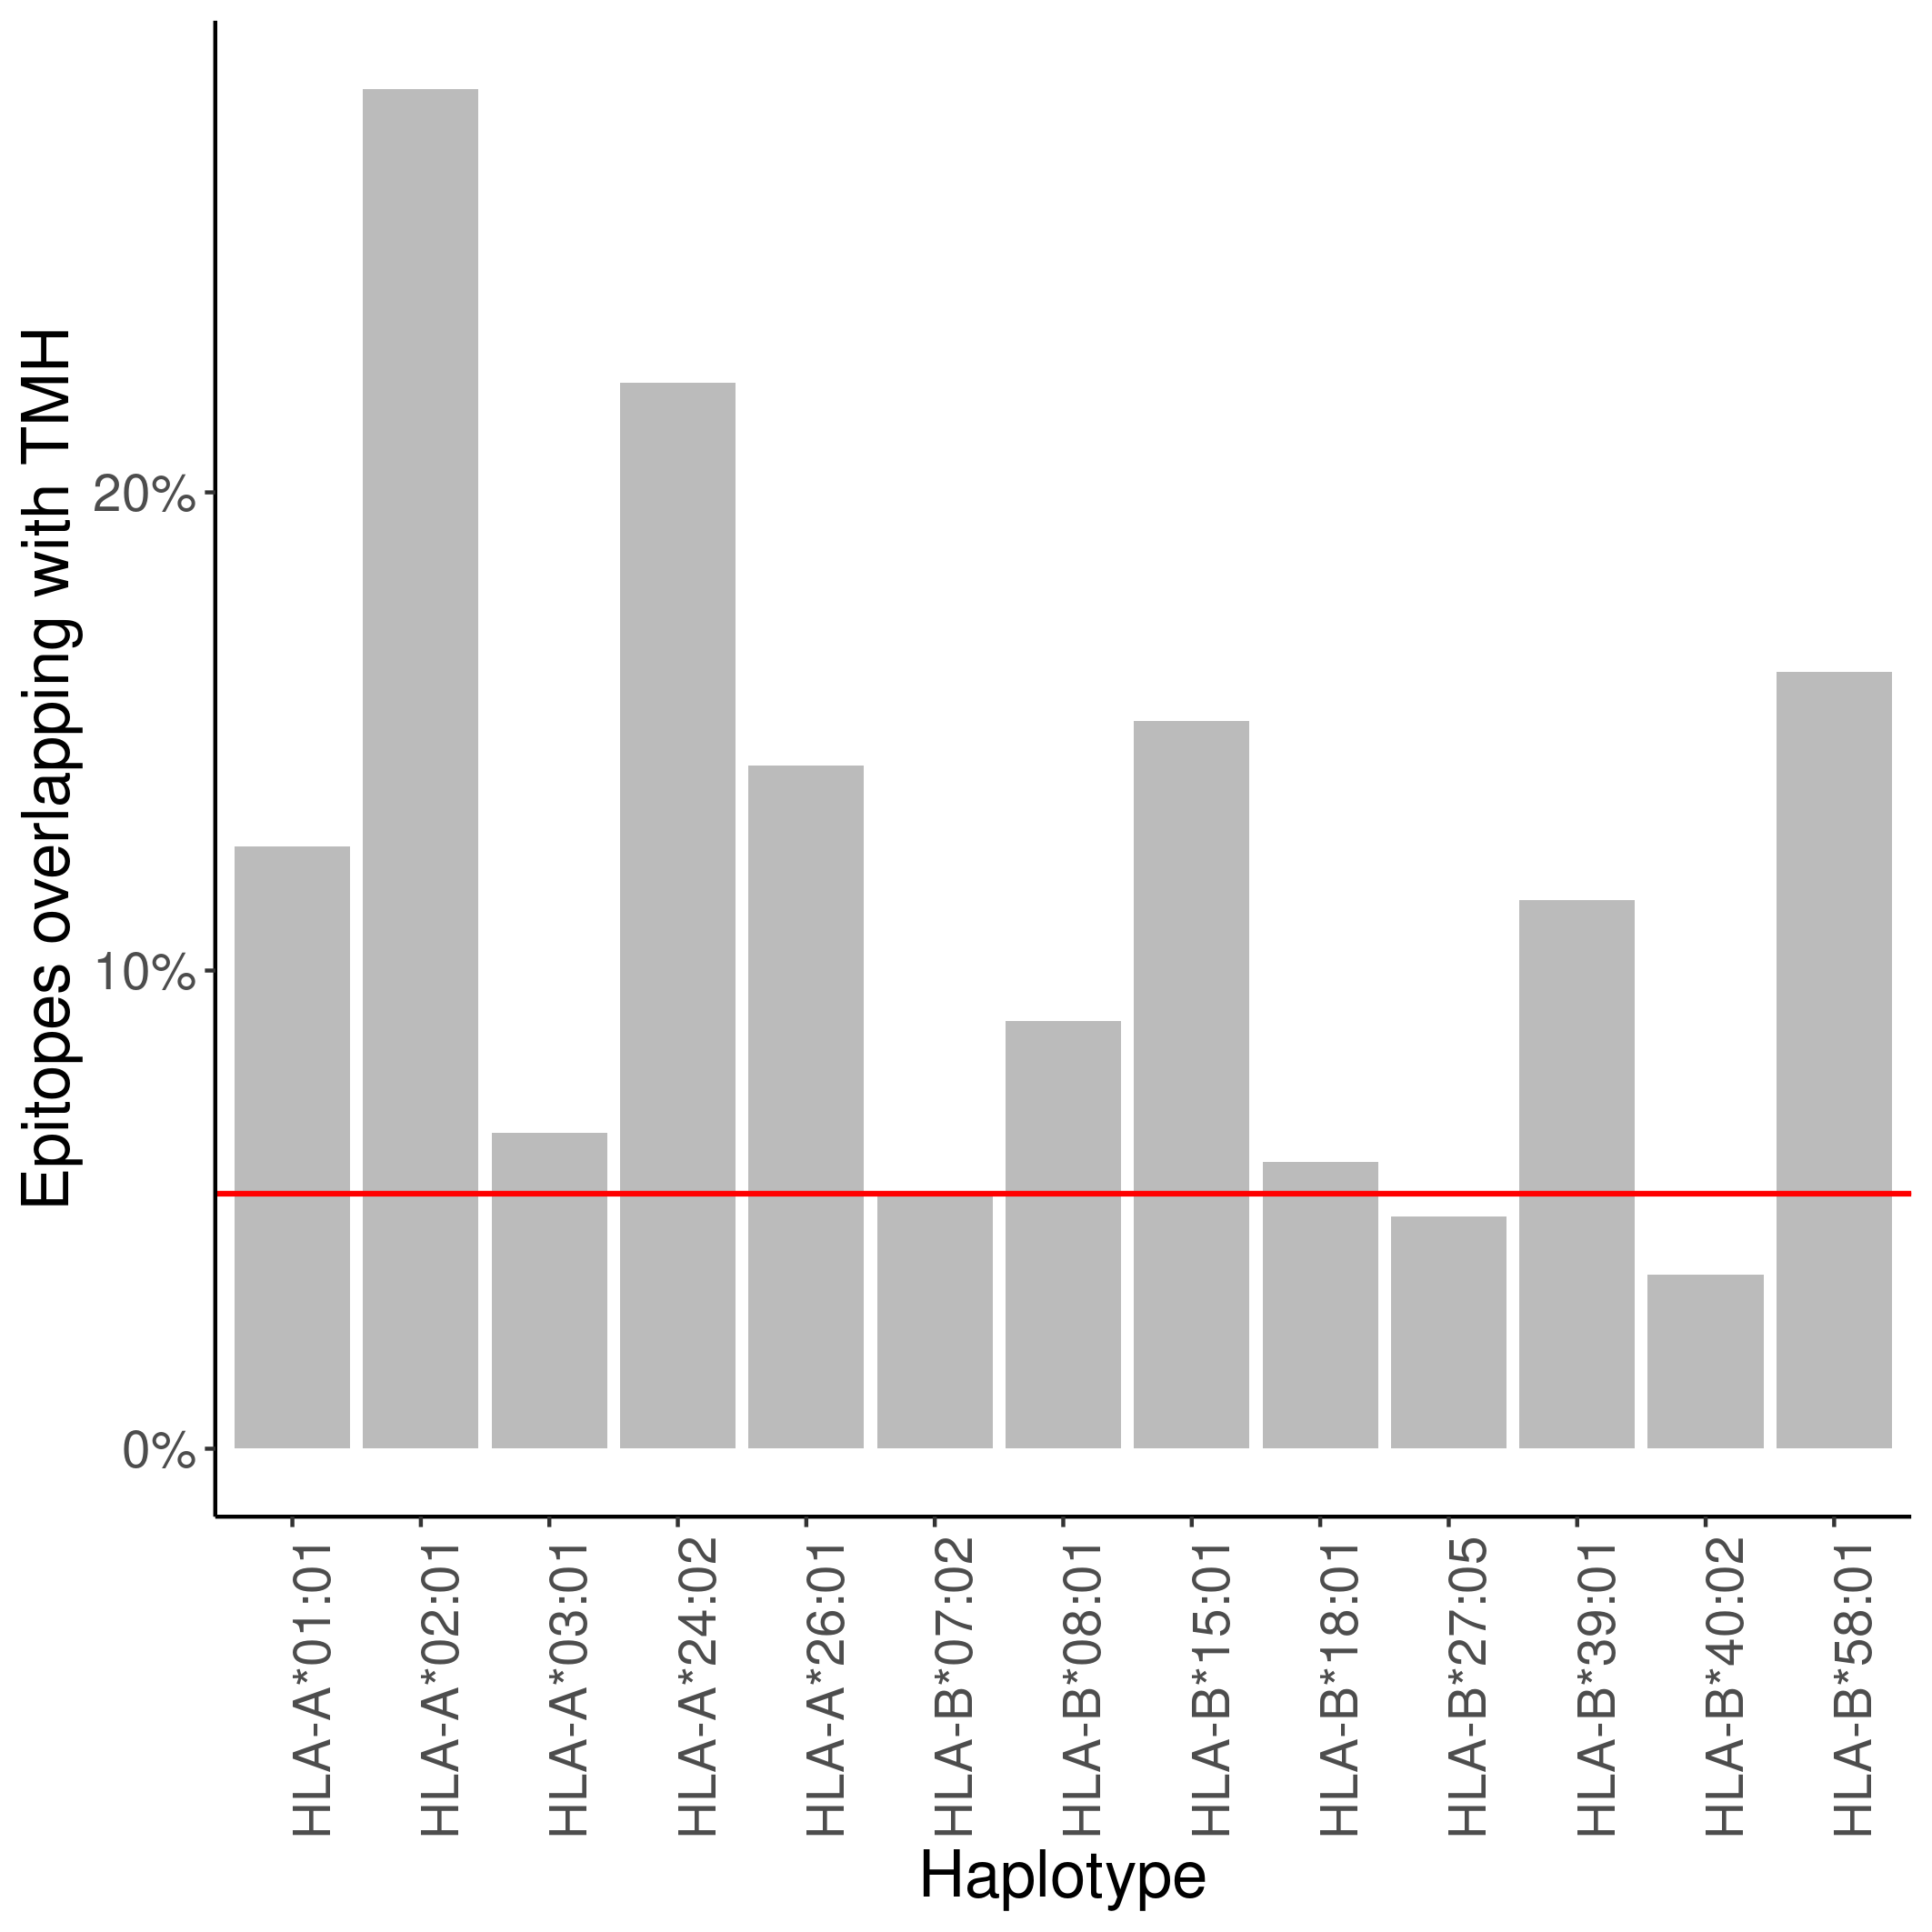
\includegraphics[width=\linewidth]{bbbq_1_smart_results/fig_f_tmh_2_human_mhc1.png}
\end{center}
\caption{
    Results for this study.
    Dashed line denotes the percentage as expected by chance.
}
\label{fig:bilderbeek_et_al_2021_1a}
\end{figure}

% Process all floats before going to a next page
\clearpage

%%%%%%%%%%%%%%%%%%%%%%%%%%%%%%%%%%%%%%%%%%%%%%%%%%%%%%%%%%%%%%%%%%%%%%%%%%%%%%%%
\section{IC50 values of binders per MHC allele}
\label{subsec:ic50s_per_haplotype}
%%%%%%%%%%%%%%%%%%%%%%%%%%%%%%%%%%%%%%%%%%%%%%%%%%%%%%%%%%%%%%%%%%%%%%%%%%%%%%%%

Per target proteome (i.e. human, SARS-CoV-2, \emph{M tuberculosis}),
we collected all 9-mers (for MHC-I) and 14-mers (for MHC-II),
after removing the selenoproteins and proteins that are shorter
than the epitope length.
From these epitopes, per MHC allele,
we predicted the IC50 (in nM) using \verb;epitope-prediction; (for MHC-I)
and MHCnuggets (for MHC-II). 
Here, we show the IC50 value per MHC allele that
is used to determine if a peptide binds to the allele's MHC
for MHC-I (see supplementary Table \ref{tab:ic50_binders_mhc1}) and 
MHC-II (see supplementary Table \ref{tab:ic50_binders_mhc2}).

% tab:ic50_binders_mhc1
\input{bbbq_1_smart_results/table_ic50_binders_mhc1_2.latex}

% tab:ic50_binders_mhc2
\input{bbbq_1_smart_results/table_ic50_binders_mhc2_2.latex}

% Process all floats before going to a next page
\clearpage

%%%%%%%%%%%%%%%%%%%%%%%%%%%%%%%%%%%%%%%%%%%%%%%%%%%%%%%%%%%%%%%%%%%%%%%%%%%%%%%%
\section{Counts}
\label{subsec:counts}
%%%%%%%%%%%%%%%%%%%%%%%%%%%%%%%%%%%%%%%%%%%%%%%%%%%%%%%%%%%%%%%%%%%%%%%%%%%%%%%%

See supplementary Tables \ref{tab:ncbi_counts_1} and \ref{tab:ncbi_counts_2}
for an overview of all amounts. 
Note that, for the analyses using the SARS-CoV-2 virus proteome,
we labeled this by its disease (\verb;covid;) to prevent typos.
In supplementary Table \ref{tab:ncbi_counts_1} there are multiple instances where
the amounts are expected to add up, yet don't, as one SNP can work on
multiple isoforms. For example, there are 9,621 unique SNPs 
found in all proteins, of which 4,219 around found in MAPs 
and 6,026 in TMPs. Apparently, 624 SNPs work on a set of isoforms that
contains both MAPs and TMPs.

% Label: tab:ncbi_counts_1
\begin{table}

\caption{\label{tab:ncbi_counts_1}Amounts. raw = all variations, including DNA variations. all\_proteins = all proteins. map = membrane associated protein. tmp = transmembrane protein. in\_tmh = in transmembrane helix of TMP. in\_sol = in soluble region of TMP. }
\centering
\begin{tabular}[t]{l|r|r|r|r|r|r}
\hline
what & raw & all\_proteins & map & tmp & in\_tmh & in\_sol\\
\hline
Number of variations & 60931 & 37831 & 16623 & 21208 & 3803 & 17405\\
\hline
Number of unique variations & 60544 & 37630 & 16606 & 21024 & 3789 & 17235\\
\hline
Number of unique SNPs & NA & 9621 & 4219 & 6026 & 1140 & 4936\\
\hline
Number of unique gene names & 953 & 911 & 457 & 605 & 325 & 590\\
\hline
Number of unique protein names & 5163 & 4780 & 2227 & 2553 & 1280 & 2467\\
\hline
Percentage TMH & NA & 10 & 0 & 19 & 26 & 18\\
\hline
\end{tabular}
\end{table}

% Label: tab:ncbi_counts_2
\begin{table}

\caption{\label{tab:ncbi_counts_2}Amounts. single\_in\_tmh = in transmembrane helix of single-spanner. single\_in\_sol = in soluble region of single-spanner. multi\_in\_tmh = in transmembrane helix of multi-spanner. multi\_in\_sol = in soluble region of multi-spanner. }
\centering
\begin{tabular}[t]{l|r|r|r|r}
\hline
what & single\_in\_tmh & single\_in\_sol & multi\_in\_tmh & multi\_in\_sol\\
\hline
Number of variations & 452 & 7734 & 3351 & 9671\\
\hline
Number of unique variations & 451 & 7733 & 3338 & 9502\\
\hline
Number of unique SNPs & 160 & 2393 & 994 & 2762\\
\hline
Number of unique gene names & 96 & 282 & 243 & 344\\
\hline
Number of unique protein names & 304 & 1032 & 976 & 1435\\
\hline
Percentage TMH & 11 & 5 & 35 & 26\\
\hline
\end{tabular}
\end{table}

% Process all floats before going to a next page
\clearpage

%%%%%%%%%%%%%%%%%%%%%%%%%%%%%%%%%%%%%%%%%%%%%%%%%%%%%%%%%%%%%%%%%%%%%%%%%%%%%%%%
\section{Relative positions}
%%%%%%%%%%%%%%%%%%%%%%%%%%%%%%%%%%%%%%%%%%%%%%%%%%%%%%%%%%%%%%%%%%%%%%%%%%%%%%%%

See Supplementary Figure \ref{fig:snp_rel_pos}
for the distribution of the relative position of the SNPs.

\begin{figure}[!htbp]
  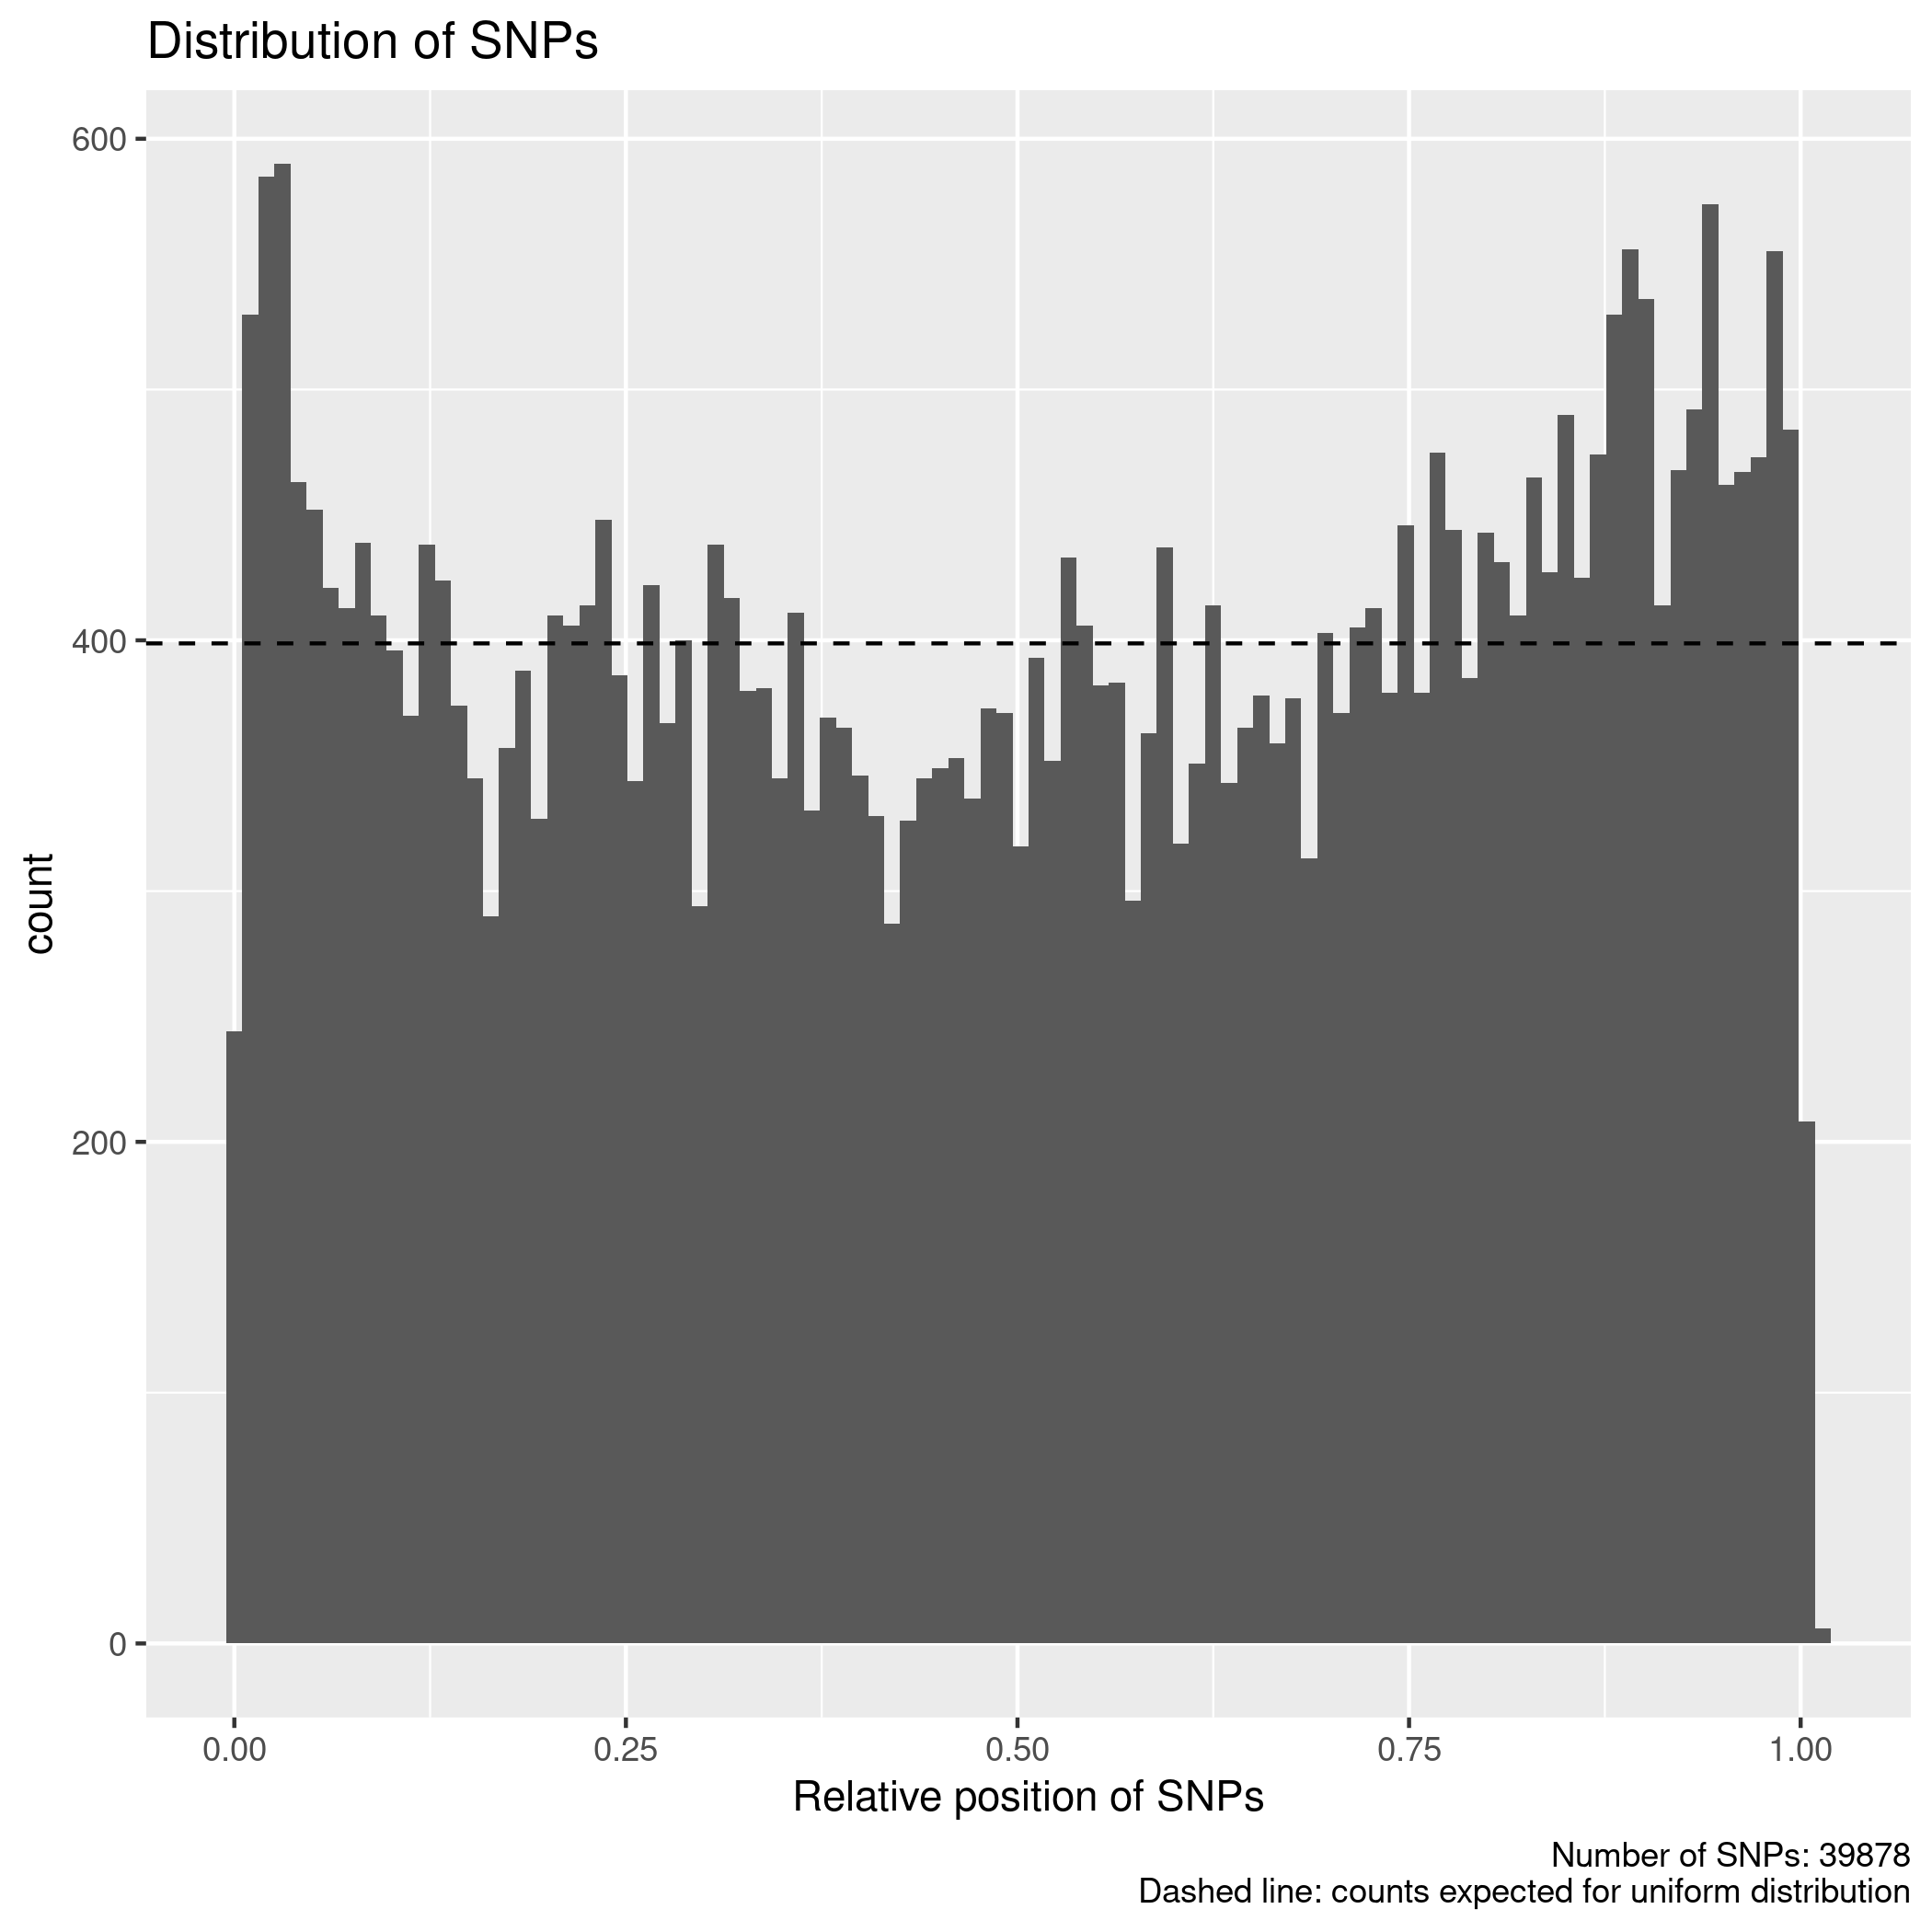
\includegraphics[width=\textwidth]{ncbi_peregrine_results/fig_snp_rel_pos.png}
  \caption{
    Distribution of the relative position of the SNPs used,
    where a relative position of zero denotes the first amino
    acid at the N-terminus, where a relative position of one
    indicates the last residue at the C-terminus.
  }
  \label{fig:snp_rel_pos}
\end{figure}

% Process all floats before going to a next page
\clearpage

%%%%%%%%%%%%%%%%%%%%%%%%%%%%%%%%%%%%%%%%%%%%%%%%%%%%%%%%%%%%%%%%%%%%%%%%%%%%%%%%
\section{Presentation of TMH-derived epitopes}
%%%%%%%%%%%%%%%%%%%%%%%%%%%%%%%%%%%%%%%%%%%%%%%%%%%%%%%%%%%%%%%%%%%%%%%%%%%%%%%%

See supplementary Table \ref{tab:tmh_binders_mhc2} 
for the percentage of MHC-II 14-mers overlapping with TMH.

% Label: tab:tmh_binders_mhc2
\input{bbbq_1_smart_results/table_tmh_binders_mhc2_2.latex}

% Process all floats before going to a next page
\clearpage

%%%%%%%%%%%%%%%%%%%%%%%%%%%%%%%%%%%%%%%%%%%%%%%%%%%%%%%%%%%%%%%%%%%%%%%%%%%%
\section{The percentage of TMH-derived epitopes from IEDB epitopes}
%%%%%%%%%%%%%%%%%%%%%%%%%%%%%%%%%%%%%%%%%%%%%%%%%%%%%%%%%%%%%%%%%%%%%%%%%%%%

We display the over-presentation of epitopes taken from the
IEDB database, for two assays: an MHC ligand assay (Figure 2A)
and a T cell assay (see figure \ref{fig:t_cells_present_tmh_derived_epitopes}),
as a bar plot.
Supplementary Table \ref{tab:elution} below shows the
exact numbers.

% tab:elution
% latex table generated in R 4.1.1 by xtable 1.8-4 package
% Fri Oct 29 12:40:25 2021
\begin{table}[ht]
\centering
\begin{tabular}{llll}
  \hline
MHC class & Tool & Dataset & n \\ 
  \hline
I & PureseqTM & schellens & 1.38\% (109/7897) \\ 
  I & PureseqTM & iedb & 6.81\% (43/631) \\ 
  I & TMHMM & schellens & 1.43\% (113/7897) \\ 
  I & TMHMM & iedb & 7.13\% (45/631) \\ 
  II & PureseqTM & bergseng & 3.92\% (498/12712) \\ 
  II & PureseqTM & iedb & 0.29\% (4/1364) \\ 
  II & TMHMM & bergseng & 3.96\% (504/12712) \\ 
  II & TMHMM & iedb & 1.39\% (19/1364) \\ 
   \hline
\end{tabular}
\caption{Percentage of epitopes derived from a TMH found in the two elution studies, for the two different kind of topology prediction tools. The values between braces show the the number of epitopes that were predicted to overlapping with a TMH per all epitopes that could be uniquely mapped to the representative human reference proteome.} 
\label{tab:elution}
\end{table}


% Process all floats before going to a next page
\clearpage



%%%%%%%%%%%%%%%%%%%%%%%%%%%%%%%%%%%%%%%%%%%%%%%%%%%%%%%%%%%%%%%%%%%%%%%%%%%%%%%%
\section{Correlation of epitope presentation}
%%%%%%%%%%%%%%%%%%%%%%%%%%%%%%%%%%%%%%%%%%%%%%%%%%%%%%%%%%%%%%%%%%%%%%%%%%%%%%%%

In the main text of this research, we use two sources of epitopes
to determine if TMH-derived epitopes are presented.
The first source of epitopes are all the 9-mers (for MHC-I) (and 14-mers for MHC-II)
derived from a human reference proteome, where this over-presentation
is displayed in figure 1A.
The second source of epitopes are those that are present in the IEDB
that are obtained from MHC ligand assays,
as displayed in figure 2A.

Here we correlate between the over-presentation of TMH-derived
epitopes between these two sources of data.
Figure \ref{fig:thm_presentation_correlation} shows per MHC allele
the percentage of TMH-derived epitopes, with a linear trendline.

\begin{figure}[!htbp]
  \centering
  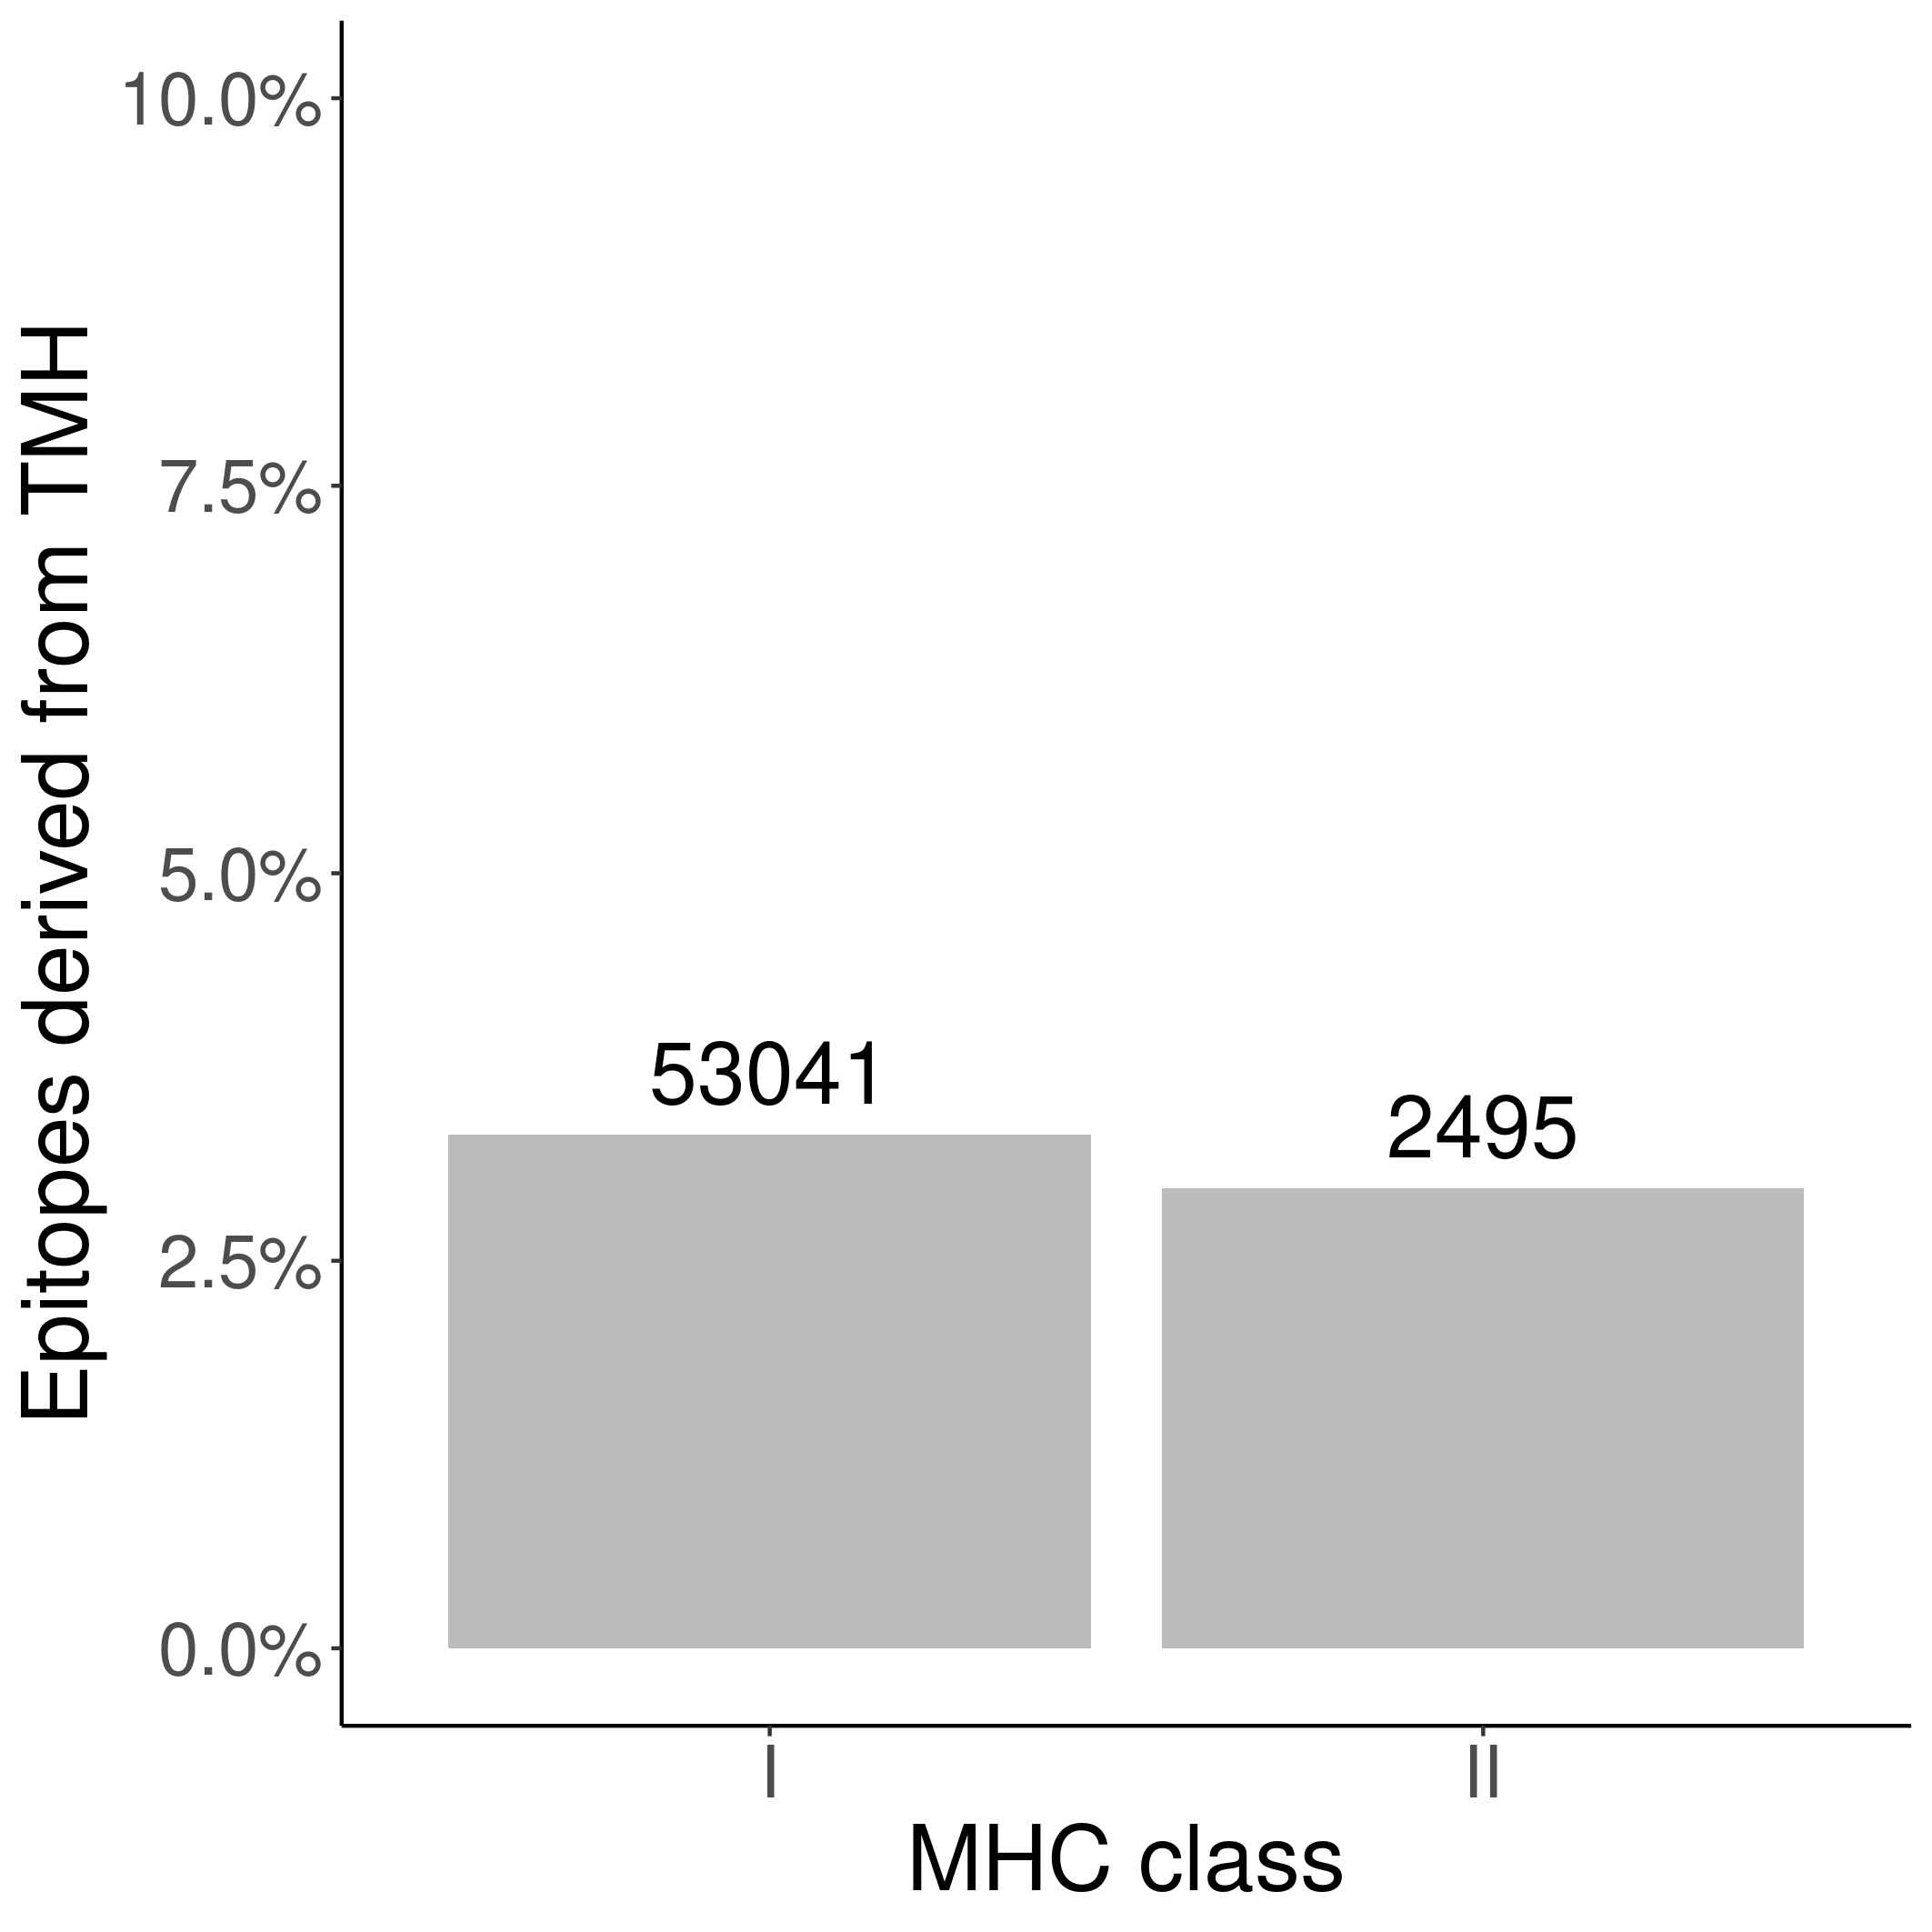
\includegraphics[width=0.5\textwidth]{bbbq_article_issue_157/figure_2c.png}
  \caption{
    \textbf{
      TMH-derived epitopes are over-presented when using
      predicted as well as experimental data
    }
    For the MHC class I alleles, the over-presentation of
    TMH-derived epitopes is correlated between 
    IEDB MHC ligand epitopes (horizontal axis) and the 9-mers
    derived from a human reference proteome (vertical axis).
    Alleles are listed in Table \ref{tab:haplotype_abbreviations}).
    The trendline shows the linear correlation between these
    percentages, where the gray area is the 95\% confidence interval.
  }
  \label{fig:thm_presentation_correlation}
\end{figure}

% Process all floats before going to a next page
\clearpage

%%%%%%%%%%%%%%%%%%%%%%%%%%%%%%%%%%%%%%%%%%%%%%%%%%%%%%%%%%%%%%%%%%%%%%%%%%%%%%%%
\section{Presentation of TMH-derived epitopes result in T cell responses}
%%%%%%%%%%%%%%%%%%%%%%%%%%%%%%%%%%%%%%%%%%%%%%%%%%%%%%%%%%%%%%%%%%%%%%%%%%%%%%%%

Figure \ref{fig:t_cells_present_tmh_derived_epitopes} 
shows the percentage of TMH-derived
epitopes of the reported epitopes from human origin for which T-cell responses were established. 
The data was obtained from the IEDB and includes only the MHC
alleles used in this study. As there are many (especially class II)
MHC alleles, only a small percentage of the full IEDB data could be used.


\begin{figure}[!htbp]
  \centering
  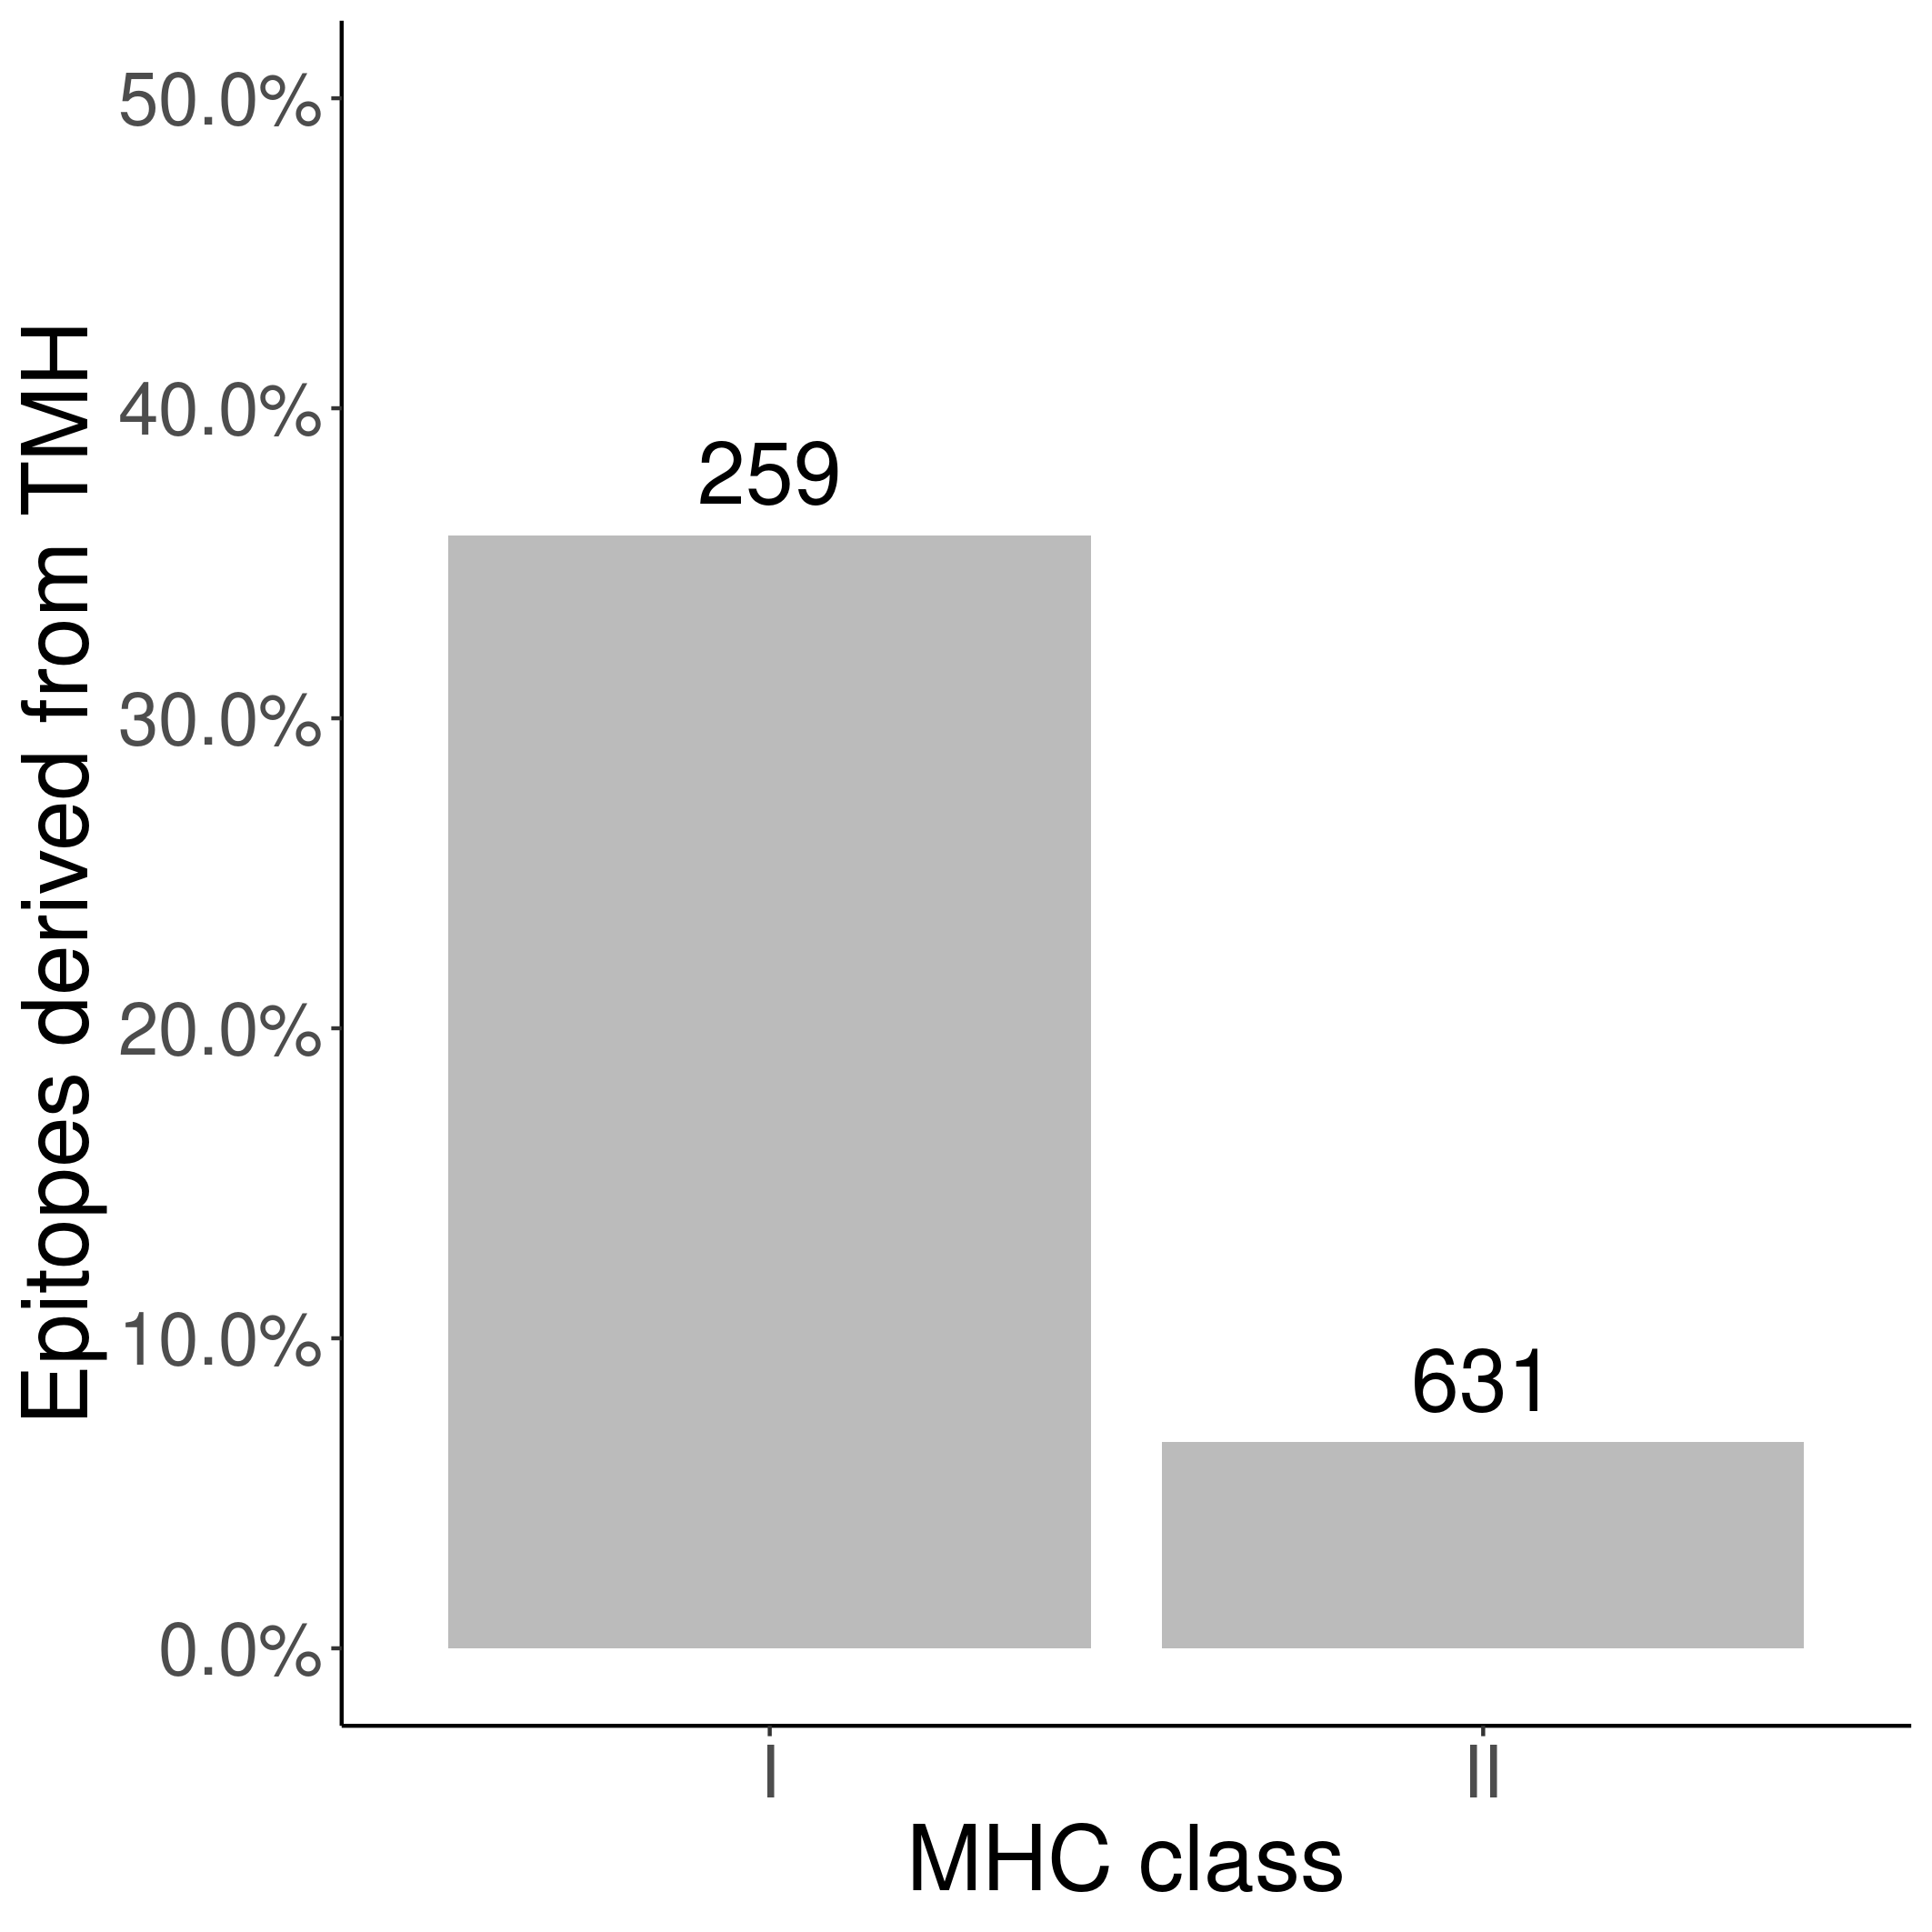
\includegraphics[width=0.5\textwidth]{bbbq_article_issue_157/figure_2d.png}
  \caption{
    \textbf{
      TMH-derived epitopes evoke T-cell responses 
      }
    The numbers above the bars denotes the number of epitopes
    found in the IEDB for the MHC alleles used in this study.
  }
  \label{fig:t_cells_present_tmh_derived_epitopes}
\end{figure}

% Process all floats before going to a next page
\clearpage

%%%%%%%%%%%%%%%%%%%%%%%%%%%%%%%%%%%%%%%%%%%%%%%%%%%%%%%%%%%%%%%%%%%%%%%%%%%%%%%%
\section{Presentation of TMH-derived epitopes}
%%%%%%%%%%%%%%%%%%%%%%%%%%%%%%%%%%%%%%%%%%%%%%%%%%%%%%%%%%%%%%%%%%%%%%%%%%%%%%%%

See supplementary Table \ref{tab:tmh_binders_mhc1} 
for the percentage of MHC-I 9-mers overlapping with TMH.

% Label: tab:tmh_binders_mhc1
\input{bbbq_1_smart_results/table_tmh_binders_mhc1_2.latex}

Supplementary Table \ref{tab:haplotype_abbreviations} shows the
shorthand notation for the HLA alleles.

% Label: tab:haplotype_abbreviations
% latex table generated in R 4.0.4 by xtable 1.8-4 package
% Mon Apr  5 12:14:41 2021
\begin{table}[ht]
\centering
\begin{tabular}{rl}
  \hline
index & haplotype\_name \\ 
  \hline
  1 & HLA-A*01:01 \\ 
    2 & HLA-A*02:01 \\ 
    3 & HLA-A*03:01 \\ 
    4 & HLA-A*24:02 \\ 
    5 & HLA-A*26:01 \\ 
    6 & HLA-B*07:02 \\ 
    7 & HLA-B*08:01 \\ 
    8 & HLA-B*18:01 \\ 
    9 & HLA-B*27:05 \\ 
   10 & HLA-B*39:01 \\ 
   11 & HLA-B*40:02 \\ 
   12 & HLA-B*58:01 \\ 
   13 & HLA-B*15:01 \\ 
    1 & HLA-DRB1*0101 \\ 
    2 & HLA-DRB1*0301 \\ 
    3 & HLA-DRB1*0401 \\ 
    4 & HLA-DRB1*0405 \\ 
    5 & HLA-DRB1*0701 \\ 
    6 & HLA-DRB1*0802 \\ 
    7 & HLA-DRB1*0901 \\ 
    8 & HLA-DRB1*1101 \\ 
    9 & HLA-DRB1*1201 \\ 
   10 & HLA-DRB1*1302 \\ 
   11 & HLA-DRB1*1501 \\ 
   12 & HLA-DRB3*0101 \\ 
   13 & HLA-DRB3*0202 \\ 
   14 & HLA-DRB4*0101 \\ 
   15 & HLA-DRB5*0101 \\ 
   16 & HLA-DQA1*0501/DQB1*0201 \\ 
   17 & HLA-DQA1*0501/DQB1*0301 \\ 
   18 & HLA-DQA1*0301/DQB1*0302 \\ 
   19 & HLA-DQA1*0401/DQB1*0402 \\ 
   20 & HLA-DQA1*0101/DQB1*0501 \\ 
   21 & HLA-DQA1*0102/DQB1*0602 \\ 
   \hline
\end{tabular}
\caption{Abbreviations of the haplotype names} 
\label{tab:haplotype_abbreviations}
\end{table}


Supplementary Tables \ref{tab:tmh_binders_mhc1} and \ref{tab:tmh_binders_mhc2}
show the exact number of binders, binders that overlap with TMHs
and the percentage of binders that overlap with TMHs, as
visualized by figure 1A.

% Process all floats before going to a next page
\clearpage

%%%%%%%%%%%%%%%%%%%%%%%%%%%%%%%%%%%%%%%%%%%%%%%%%%%%%%%%%%%%%%%%%%%%%%%%%%%%%%%%
\section{Prediction software used}
\label{subsec:prediction_software_used}
%%%%%%%%%%%%%%%%%%%%%%%%%%%%%%%%%%%%%%%%%%%%%%%%%%%%%%%%%%%%%%%%%%%%%%%%%%%%%%%%

\begin{table}[]
  \begin{tabular}{llll}
    Goal & Tool & Reference \\ 
    \hline
    Predict topology                  & TMHMM                     & \citep{krogh2001predicting} \\
    Predict topology                  & PureseqTM                 & \citep{wang2019efficient} \\
    Predict epitopes MHC-I            & \verb;epitope-prediction; & \citep{bianchi2017} \\
    Predict epitopes MHC-II           & NetMHCIIpan               & \citep{nielsen2008quantitative,karosiene2013netmhciipan} \\
    Call TMHMM from R                 & \verb;tmhmm;              & \citep{tmhmm} \\
    Call PureseqTM from R             & \verb;pureseqtmr;         & \citep{pureseqtmr} \\
    Call NetMHCIIpan from R           & \verb;netmhc2pan;         & \citep{netmhc2pan} \\
    Work with IEDB                    & \verb;iedbr;              & \citep{iedbr} \\
    Work with \verb;rentrez;          & \verb;sprentrez;          & \citep{sprentrez} \\
    Combine all                       & \verb;bbbq;               & \citep{bbbq}
  \end{tabular}
  \caption{
    Overview of all software used in this research.
  }
  \label{table:software_used}
\end{table}


For this research, we needed software to predict protein
topology, as well as the MHC-I and MHC-II binding affinities
of epitopes. We selected our software, by
searching the scientific literature 
to identify the most recent free and open source (FOSS) 
prediction software.
This was done by searching for papers that (1) cite older
prediction software, and (2) present a novel method to make predictions.
As a starting point, per type of prediction software,
a review paper was used (\citep{moller2001evaluation} for protein
topology, \citep{lundegaard2011prediction} for MHC-I
binding affinities and \citep{nielsen2003reliable} for MHC-II binding
affinities). 

% \paragraph{TMH prediction}

There are multiple computational tools developed to predict which
parts of a protein forms a TMH.
In 2001, multiple of such prediction tools have been compared \citep{moller2001evaluation},
of which TMHMM \citep{krogh2001predicting} turned out to be the most accurate, 
as is used in the previous study \citep{bianchi2017}.
However, TMHMM has a restrictive software license and is nearly two
decades old.
Therefore, PureseqTM \citep{wang2019efficient},
was also used in this study, which has been more recently developed
and has a free software license.

% \paragraph{MHC-I epitope prediction}

For MHC-I, there are multiple computational tools developed 
to predict epitopes. 
According to \citep{lundegaard2011prediction}, at that time,
NetMHCcons \citep{karosiene2012netmhccons} gave the best predictions.
We used the same tool as used in our earlier study, 
\verb;epitope-prediction; \citep{bianchi2017},

% \paragraph{MHC-II epitope prediction}

Also for MHC-II, there are multiple computational tools developed 
to predict epitopes,
such as using a trained neural network \citep{nielsen2003reliable}
or a Gibbs sampling approach \citep{nielsen2004improved}.
According to \citep{lundegaard2011prediction}, in 2011,
from a set of multiple tools, 
\mbox{NetMHCIIpan} \citep{nielsen2008quantitative,karosiene2013netmhciipan}
made the most accurate predictions.
The most recent FOSS tool available now appears
to be MHCnuggets \citep{shao2020high}, which can do both MHC-I 
and MHC-II predictions. 
As we already use \verb;epitope-prediction; \citep{bianchi2017} 
for MHC-I predictions, we use MHCnuggets only for MHC-II predictions.

% \paragraph{NCBI data retrieval software}

To retrieve the data from the NCBI databases the
\verb;rentrez; R package \citep{rentrez} was used
that calls the NCBI database's API. 
The NCBI database provides a stable user experience for all users, 
by limiting its API to 3 calls per second per user.
Additionally, the API splits the result of a bigger
query into multiple pages, each of which needs one API call.
The \verb;sprentrez; package \citep{sprentrez} provides for 
bigger queries of multiple (and delayed) API calls.

% \paragraph{IEDB software}

To retrieve the data from the IEDB  databases \citep{vita2019immune}, 
the \verb;iedbr; R package \citep{iedbr} was written,
to calls the IEDB database's API. 
Similar to the NCBI database,
the IEDB has a limit to 1 call per second per user
and allows a query results to return 10k results maximally.
The \verb;iedbr; package \citep{iedbr} allows for bigger queries.

% Process all floats before going to a next page
\clearpage

%%%%%%%%%%%%%%%%%%%%%%%%%%%%%%%%%%%%%%%%%%%%%%%%%%%%%%%%%%%%%%%%%%%%%%%%%%%%%%%%
\section{Prediction software written}
%%%%%%%%%%%%%%%%%%%%%%%%%%%%%%%%%%%%%%%%%%%%%%%%%%%%%%%%%%%%%%%%%%%%%%%%%%%%%%%%

The R programming language is used for the complete 
experiment, including the analysis.
The complete experiment is bundled in the 'bbbq' R package,
which is dependent on 'tmhmm', 'pureseqtmr', 
'epitope-prediction' and 'mhcnuggetsr'
as described below.

% \paragraph{tmhmm}

The R package 'tmhmm' was developed to do the similar topology
predictions as our earlier study (that used 'TMHMM'), yet in an automated way.
'TMHMM' has a restrictive software license \citep{krogh2001predicting} 
and allows a user
to download a pre-compiled executable after confirmation that he/she
is in academia. The R package respects this restriction
and allows the user to install and use TMHMM from within R,
as done in this study.
'tmhmm' has been submitted to and is accepted 
by the Comprehensive R Archive Network (CRAN).

% \paragraph{pureseqtmr}

To be able to call, from R, the TMH prediction 
software 'PureseqTM' \citep{wang2019efficient},
which is written in C, the package 'pureseqtmr' has been developed. 
'pureseqtmr' allows to install 'PureseqTM' and use most of its features.
'pureseqtmr' has been submitted to and is accepted by CRAN.

% \paragraph{mhcnuggetsr}

MHCnuggets is a free and open-source Python package to predict 
epitope affinity for many MHC-I and MHC-II variants \citep{shao2020high}.
The R package 'mhcnuggetsr' allows one to install and use MHCnuggets
from within R.
Also 'mhcnuggetsr' has been submitted to and is accepted by CRAN.

% \paragraph{bbbq}

To reproduce the full experiment presented in this paper,
the functions needed are bundled in the 'bbbq' R package.
This package is too specific to be submitted to CRAN.

% Process all floats before going to a next page
\clearpage

%%%%%%%%%%%%%%%%%%%%%%%%%%%%%%%%%%%%%%%%%%%%%%%%%%%%%%%%%%%%%%%%%%%%%%%%%%%%%%%%
\section{Prediction of percentage of epitopes overlapping with a TMH}
%%%%%%%%%%%%%%%%%%%%%%%%%%%%%%%%%%%%%%%%%%%%%%%%%%%%%%%%%%%%%%%%%%%%%%%%%%%%%%%%

Supplementary Table \ref{tab:f_tmh} shows an overview of the findings,
where a target specifies the source of the proteome,
where \verb;covid; denotes SARS-CoV-2 and \verb;myco; denotes
\emph{Mycobacterium tuberculosis}. \verb;mhc_class; denotes the MHC
class, \verb;n_spots; the number of possible 9-mers (for MHC-I) 
or 14-mers (for MHC-II) possible. \verb;n_spots_tmh; the
number of epitopes that overlapped with a TMH that were binders. 
\verb;f_tmh; the percentage of peptides that had at least 1 residue
overlapping with a TMH.

% Label: tab:f_tmh
\input{bbbq_1_smart_results/table_f_tmh_2.latex}

% Process all floats before going to a next page
\clearpage

%%%%%%%%%%%%%%%%%%%%%%%%%%%%%%%%%%%%%%%%%%%%%%%%%%%%%%%%%%%%%%%%%%%%%%%%%%%%%%%%
\section{Minor methods}
%%%%%%%%%%%%%%%%%%%%%%%%%%%%%%%%%%%%%%%%%%%%%%%%%%%%%%%%%%%%%%%%%%%%%%%%%%%%%%%%

These are details that are removed from the 'Methods' section.

PureseqTM does not predict the topology
of proteins that have less than three amino acids. 
The TRDD1 ('T cell receptor delta diversity 1') protein,
however, is two amino acids long. 
The R package \verb;pureseqtmr;, however, 
predicts that mono- and di-peptides are cytosolic. 

%%%%%%%%%%%%%%%%%%%%%%%%%%%%%%%%%%%%%%%%%%%%%%%%%%%%%%%%%%%%%%%%%%%%%%%%%%%%%%%%
\section{Minor discussion}
%%%%%%%%%%%%%%%%%%%%%%%%%%%%%%%%%%%%%%%%%%%%%%%%%%%%%%%%%%%%%%%%%%%%%%%%%%%%%%%%

These are details that are removed from the 'Discussion' section.

% \paragraph{Bacteria have a different cell membrane}

In this experiment we predicted epitopes that overlap with 
TMHs from a human, bacterial and viral proteome,
would these proteins be expressed in a human host.
Bacteria, however have different cell membranes and cell walls, 
hence different structural requirements for a TMH.
Both topology prediction tools were trained to recognize
human TMHs, thus we cannot be sure that
the transmembrane regions predicted in bacterial proteins
are actually part of a TMH.
For the purpose of this study, we assume the 
error in topology predictions to be unbiased way towards topology.
In other words: that a bacterial TMH is incorrectly
predicted to be absent just as often as it is incorrectly
predicted to be present elsewhere.

% \paragraph{False positives in SNPs}

Regarding the evolutionary conservation of TMHs using SNPs,
again, it is estimated that approximately ten percent
of SNPs is a false positive that result from the methods to determine
a SNP. One example is that sequence variations are incorrectly
detected due to highly similar duplicated sequences \citep{musumeci2010single}.
We assume that these duplications occur as often in TMHs as in
regions around these, hence we expect this not to affect our results.

% \paragraph{synonymous mutations}
%
In our evolutionary experiment, 
we removed variations that were synonymous mutations (i.e.
resulted in the same amino acid, from a different genetic code) 
from our analysis.
There is evidence, however, that these synonymous mutations
do have an effect and may even be evolutionary selected 
for \citep{hunt2009silent}.
As the possible effect of synonymous mutations is ignored by our
topology prediction software, we do so as well.

% Process all floats before going to a next page
\clearpage

%%%%%%%%%%%%%%%%%%%%%%%%%%%%%%%%%%%%%%%%%%%%%%%%%%%%%%%%%%%%%%%%%%%%%%%%%%%%%%%%
\section{Relative presentation of TMH-derived epitopes}
%%%%%%%%%%%%%%%%%%%%%%%%%%%%%%%%%%%%%%%%%%%%%%%%%%%%%%%%%%%%%%%%%%%%%%%%%%%%%%%%

To compare the over-presentation of TMH-derived epitopes between the
different proteomes, we normalized this percentages in such a
way that 1.0 is the percentage of TMH-derived epitopes that would 
be expected by chance. 
Figure \ref{fig:f_tmh_mhc1_normalized} and \ref{fig:f_tmh_mhc2_normalized}
show these normalized values for the MHC-I and MHC-II alleles respectively.

\begin{figure}[!htbp]
  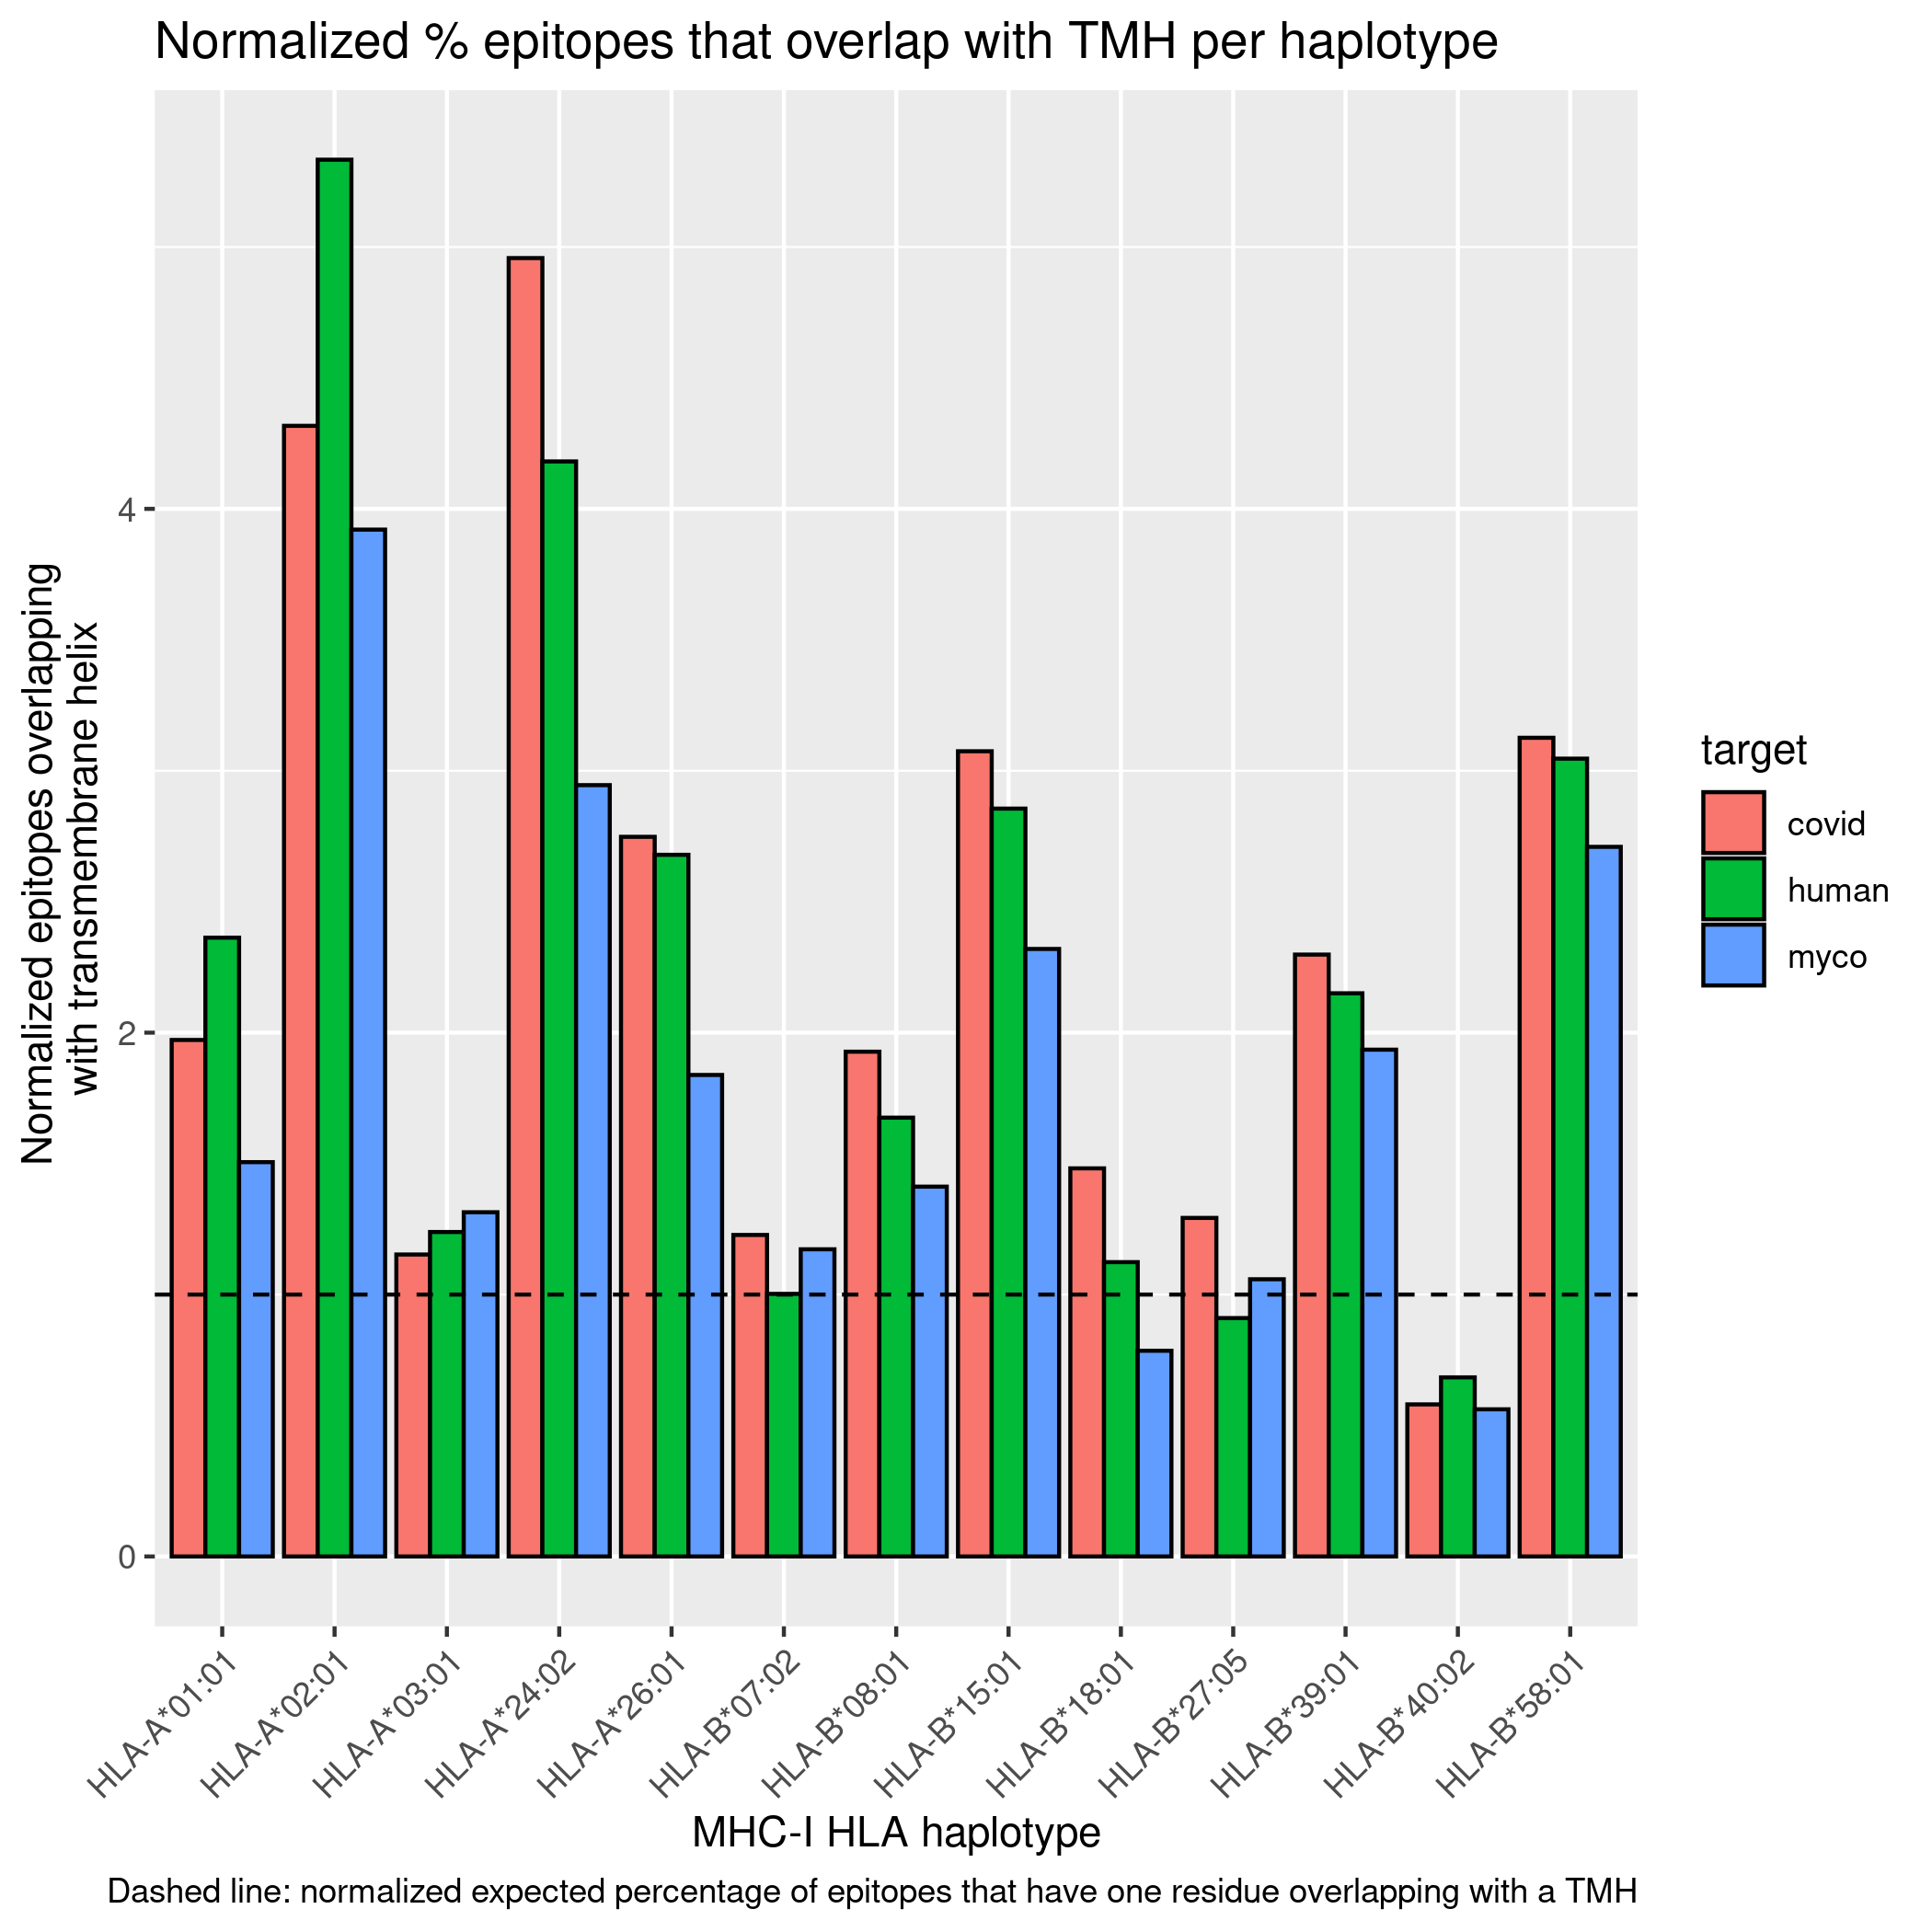
\includegraphics[width=\textwidth]{bbbq_1_smart_results/fig_f_tmh_mhc1_2_normalized.png}
  \caption{
    Normalized proportion of MHC-I epitopes overlapping with TMHs
    for human, viral and bacterial proteomes.
    Legend: covid = SARS-CoV-2,
    human = \emph{Homo sapiens}, 
    myco = \emph{Mycobacterium tuberculosis}
  }
  \label{fig:f_tmh_mhc1_normalized}
\end{figure}

\begin{figure}[!htbp]
  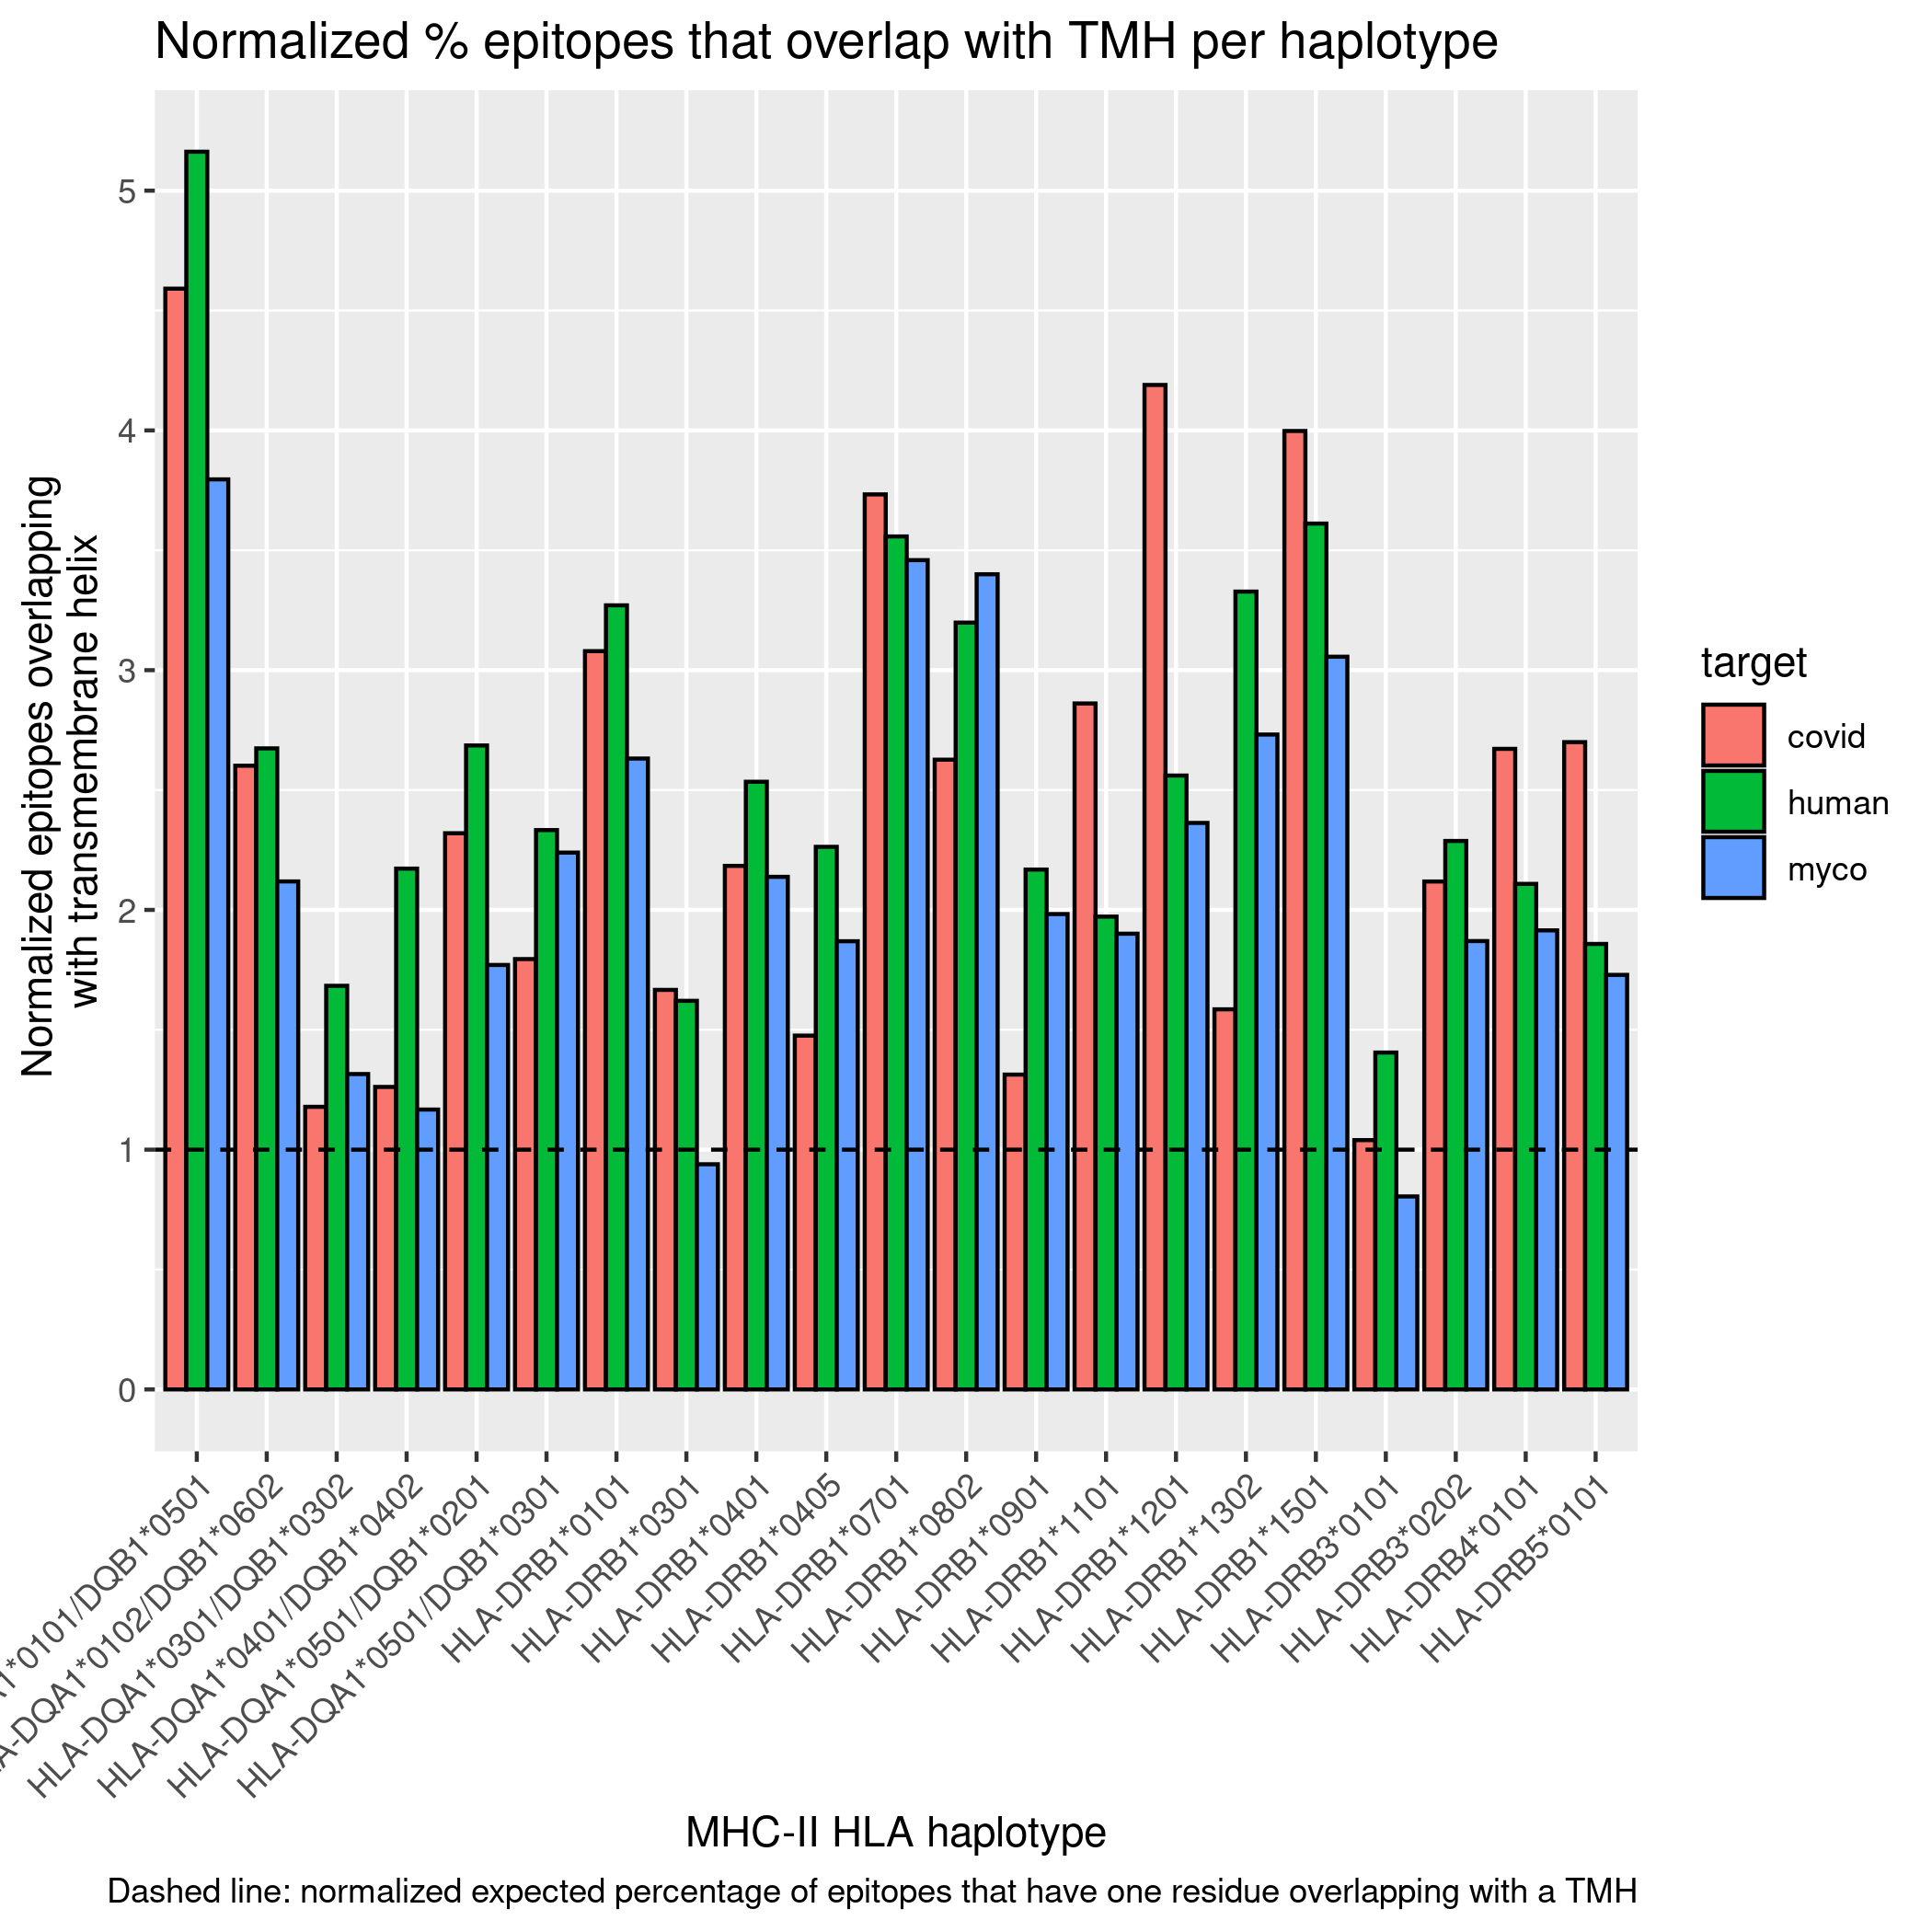
\includegraphics[width=\textwidth]{bbbq_1_smart_results/fig_f_tmh_mhc2_2_normalized.png}
  \caption{
    Normalized proportion of MHC-II epitopes overlapping with TMHs
    for human, viral and bacterial proteomes.
    Legend: covid = SARS-CoV-2,
    human = \emph{Homo sapiens}, myco = \emph{Mycobacterium tuberculosis}
  }
  \label{fig:f_tmh_mhc2_normalized}
\end{figure}

To determine the additional over-presentation of TMH-derived epitopes 
in MHC-II (as compared to MHC-I), we normalized the data to enable
a side-by-side comparison. 
The percentage of TMH-derived epitopes presented was normalized
to the expected percentage of TMH-derived epitopes,
where $1.0$ denotes that the percentage of presented TMH-derived epitopes
matches the values as expected by chance.
The normalized values per MHC allele are shown 
in figure \ref{fig:rel_presentation_per_haplotype}.
To compare the TMH-derived over-presentation per MHC class,
we grouped the normalized values per allele, 
and plot the mean and standard error, as shown in figure \ref{fig:rel_presentation}.

\begin{figure}[!htbp]
  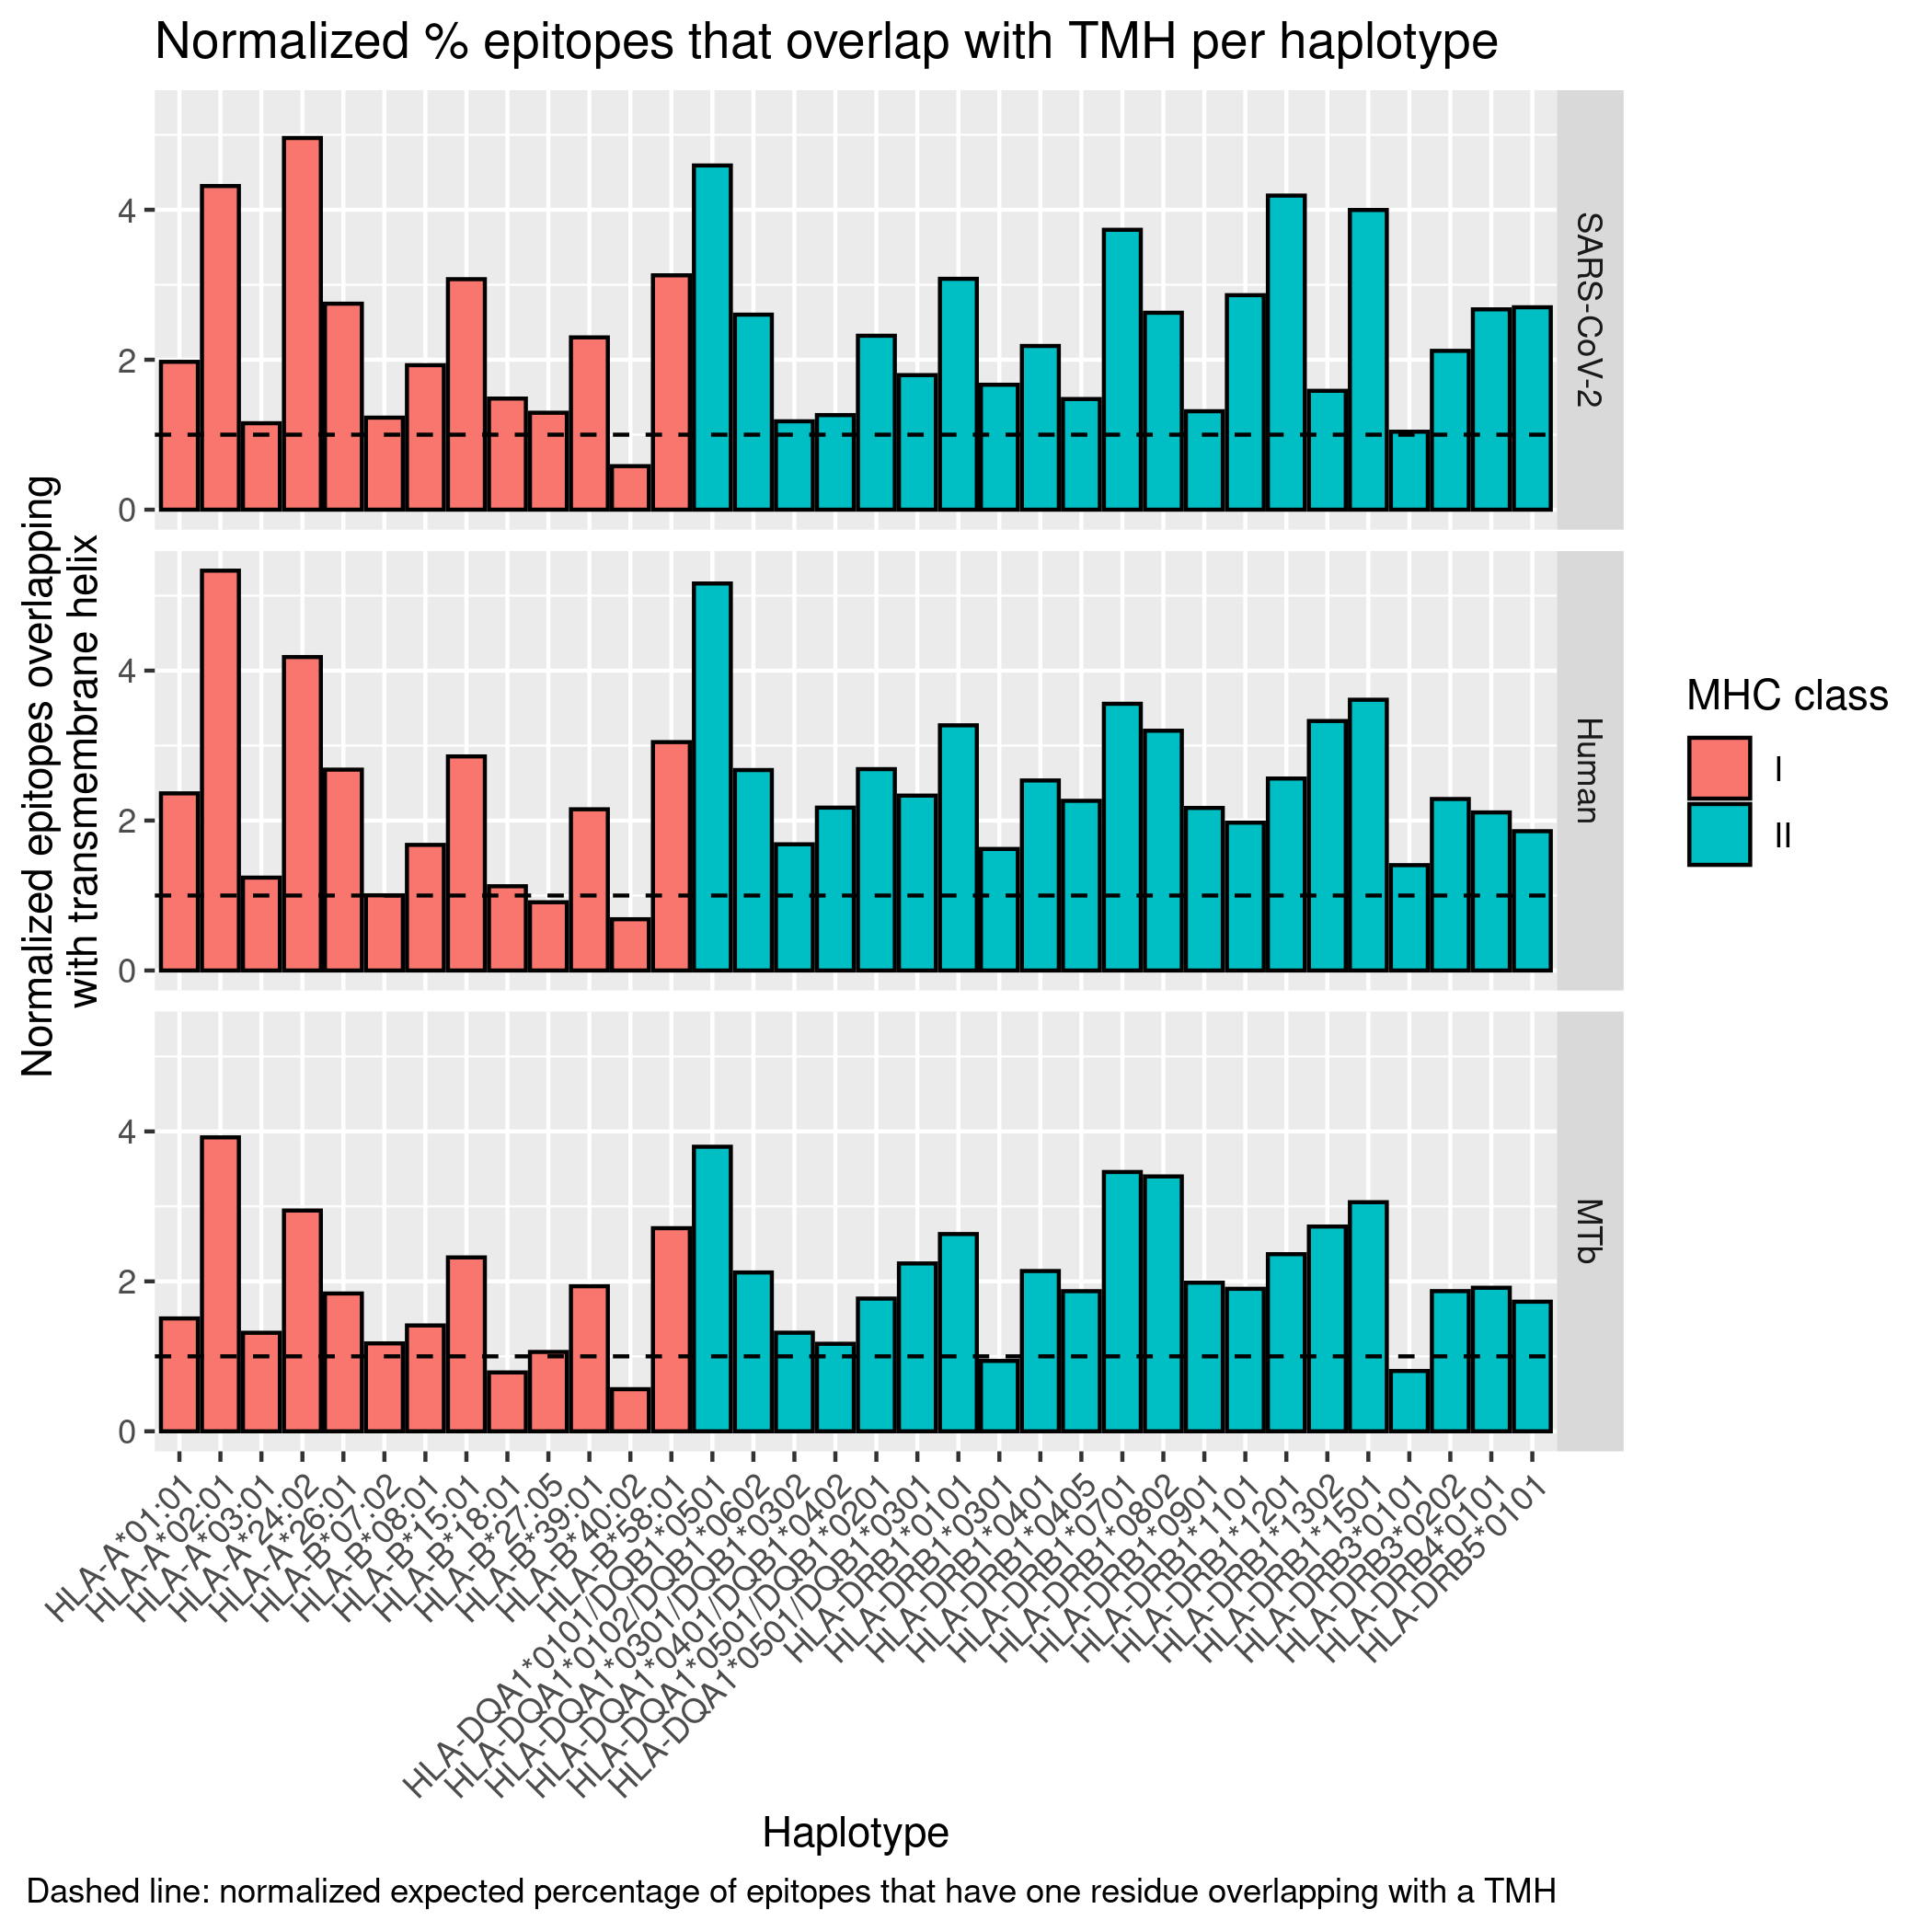
\includegraphics[width=\textwidth]{bbbq_1_smart_results/fig_rel_presentation_per_haplotype.png}
  \caption{
    Normalized proportion of MHC-I and MHC-II epitopes overlapping with TMHs,
    for the different MHC alleles and proteomes
  }
  \label{fig:rel_presentation_per_haplotype}
\end{figure}

\begin{figure}[!htbp]
  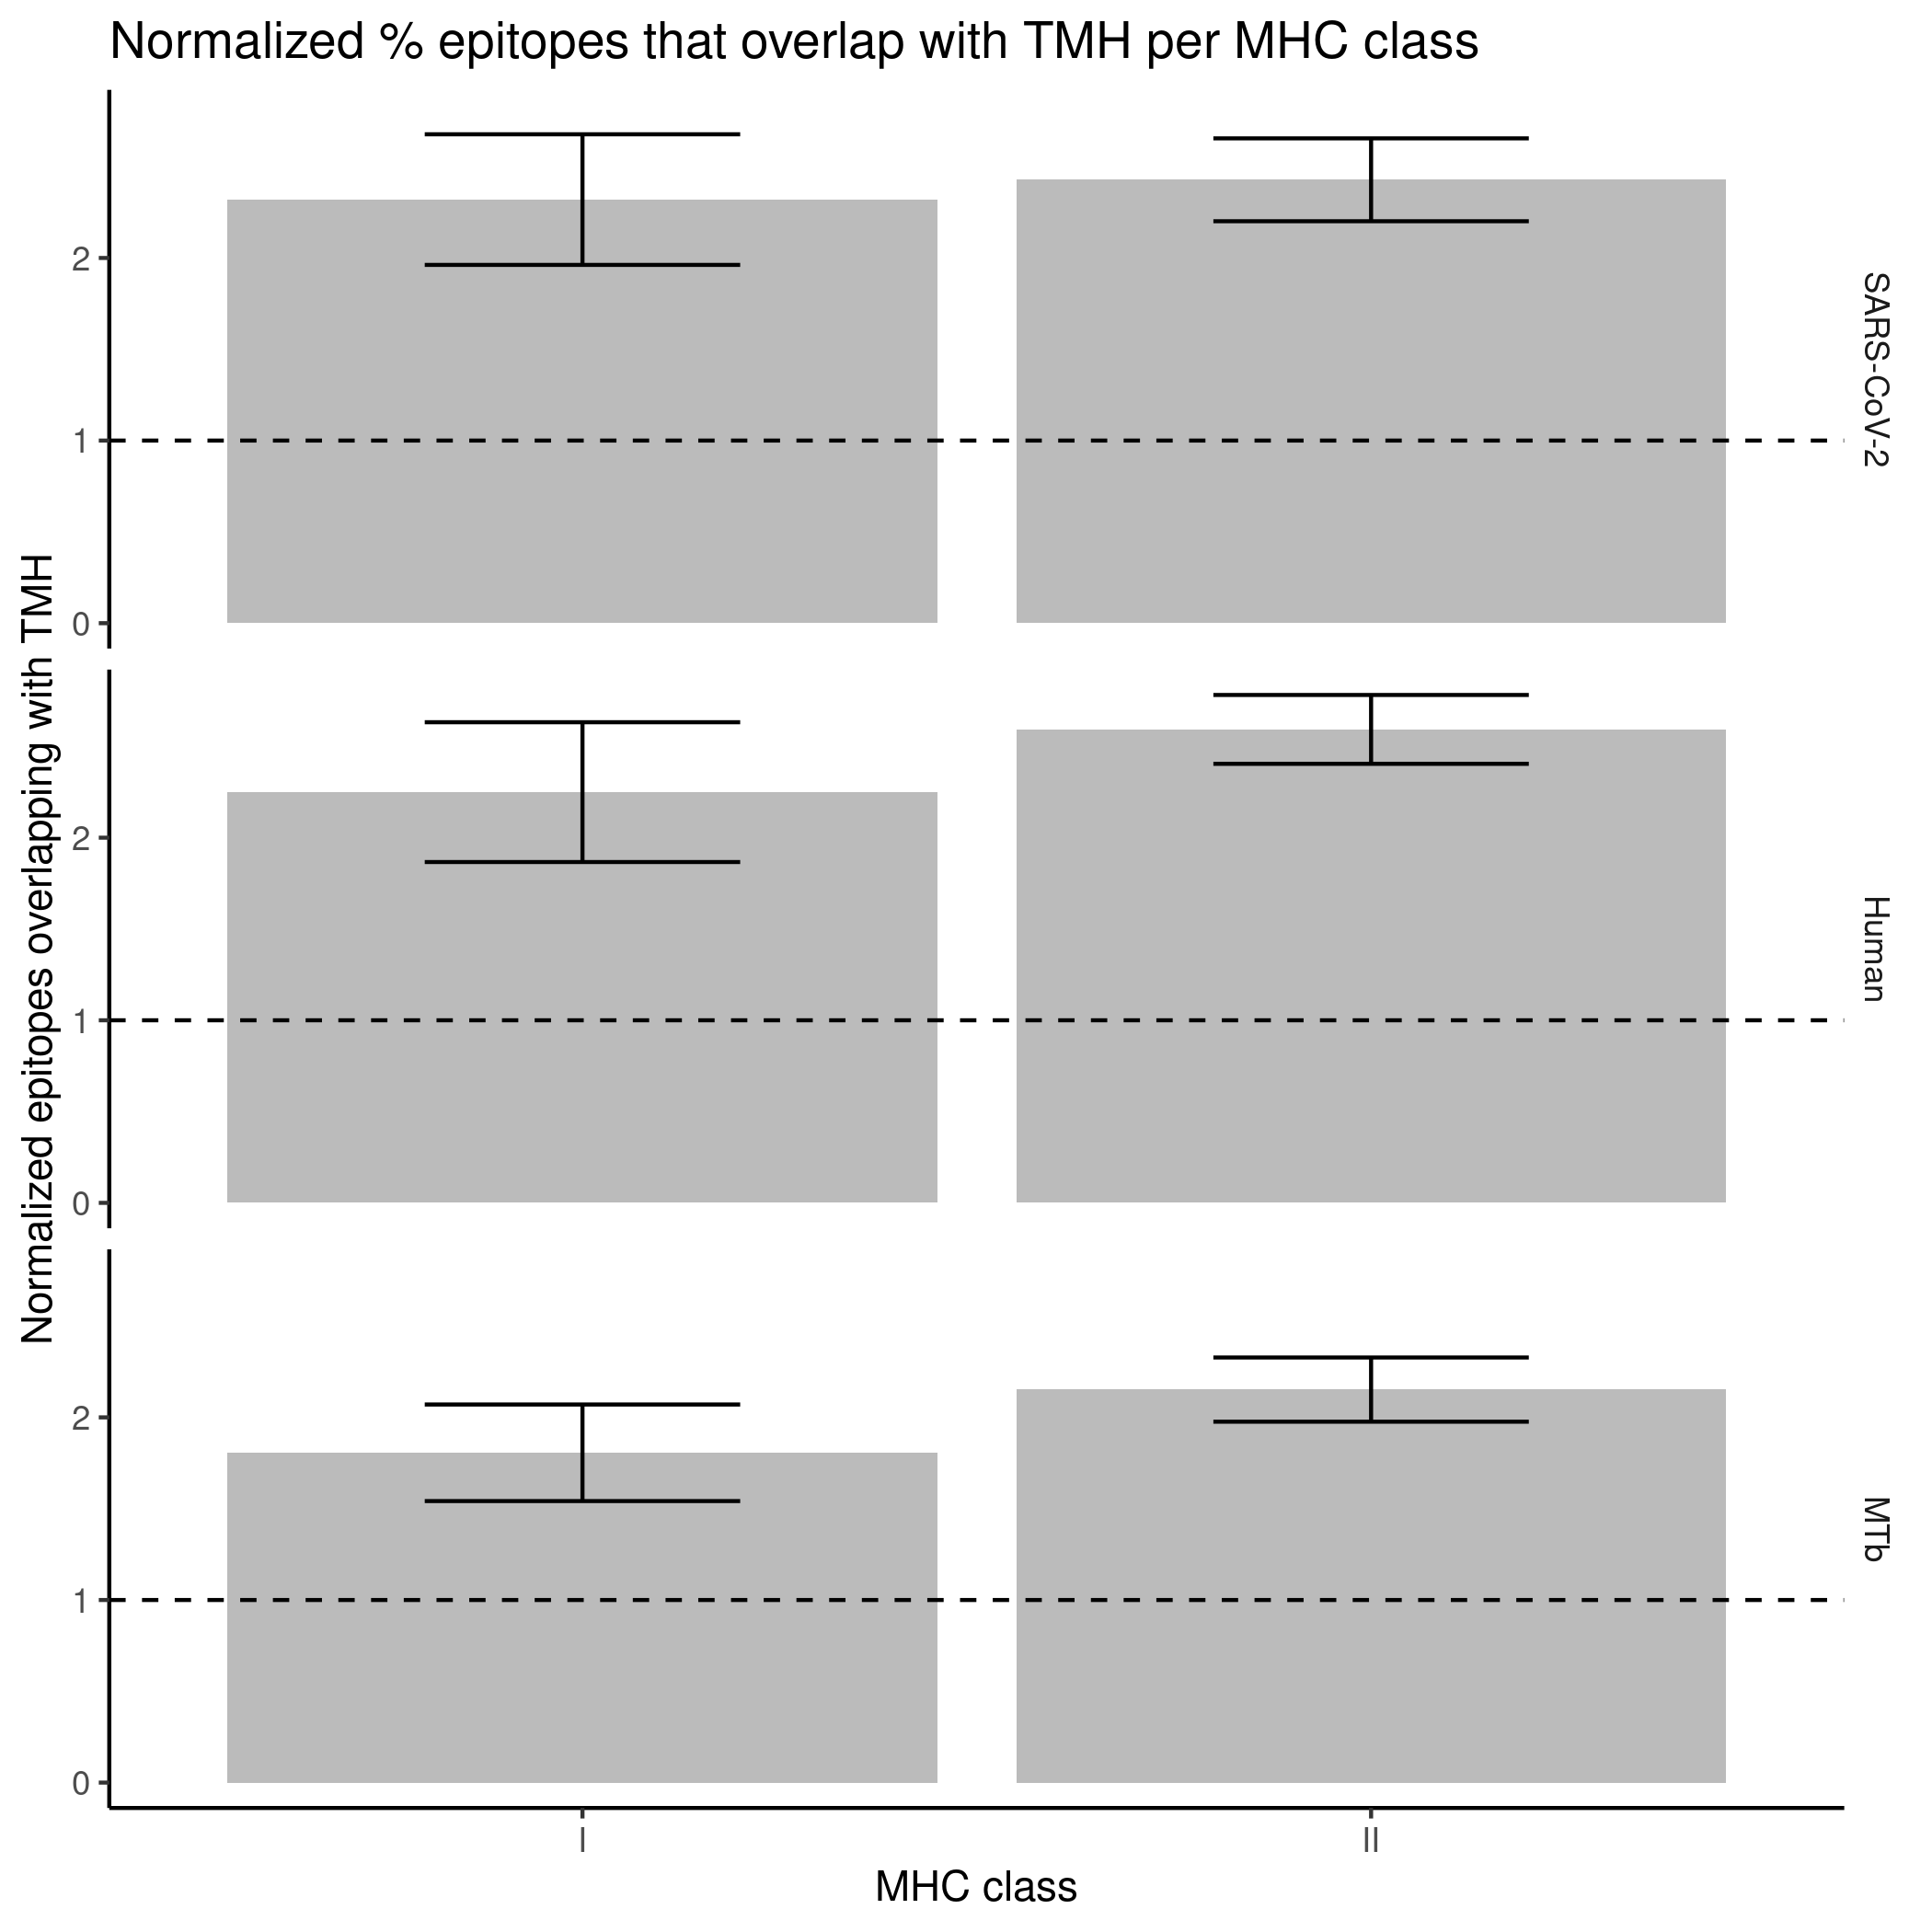
\includegraphics[width=\textwidth]{bbbq_1_smart_results/fig_rel_presentation.png}
  \caption{
    Normalized proportion of MHC-I and MHC-II epitopes overlapping with TMHs,
    for the different MHC classes and proteomes. Error bars denote the
    standard error.
  }
  \label{fig:rel_presentation}
\end{figure}

% Process all floats before going to a next page
\clearpage

%%%%%%%%%%%%%%%%%%%%%%%%%%%%%%%%%%%%%%%%%%%%%%%%%%%%%%%%%%%%%%%%%%%%%%%%%%%%%%%%
\section{Evolutionary conservation}
%%%%%%%%%%%%%%%%%%%%%%%%%%%%%%%%%%%%%%%%%%%%%%%%%%%%%%%%%%%%%%%%%%%%%%%%%%%%%%%%

Figure \ref{fig:snps_per_gene_name_ncbi} shows the distribution of the
number of SNPs per gene name, at the date we started the experiment,
at December 14th 2020.

\begin{figure}[!htbp]
  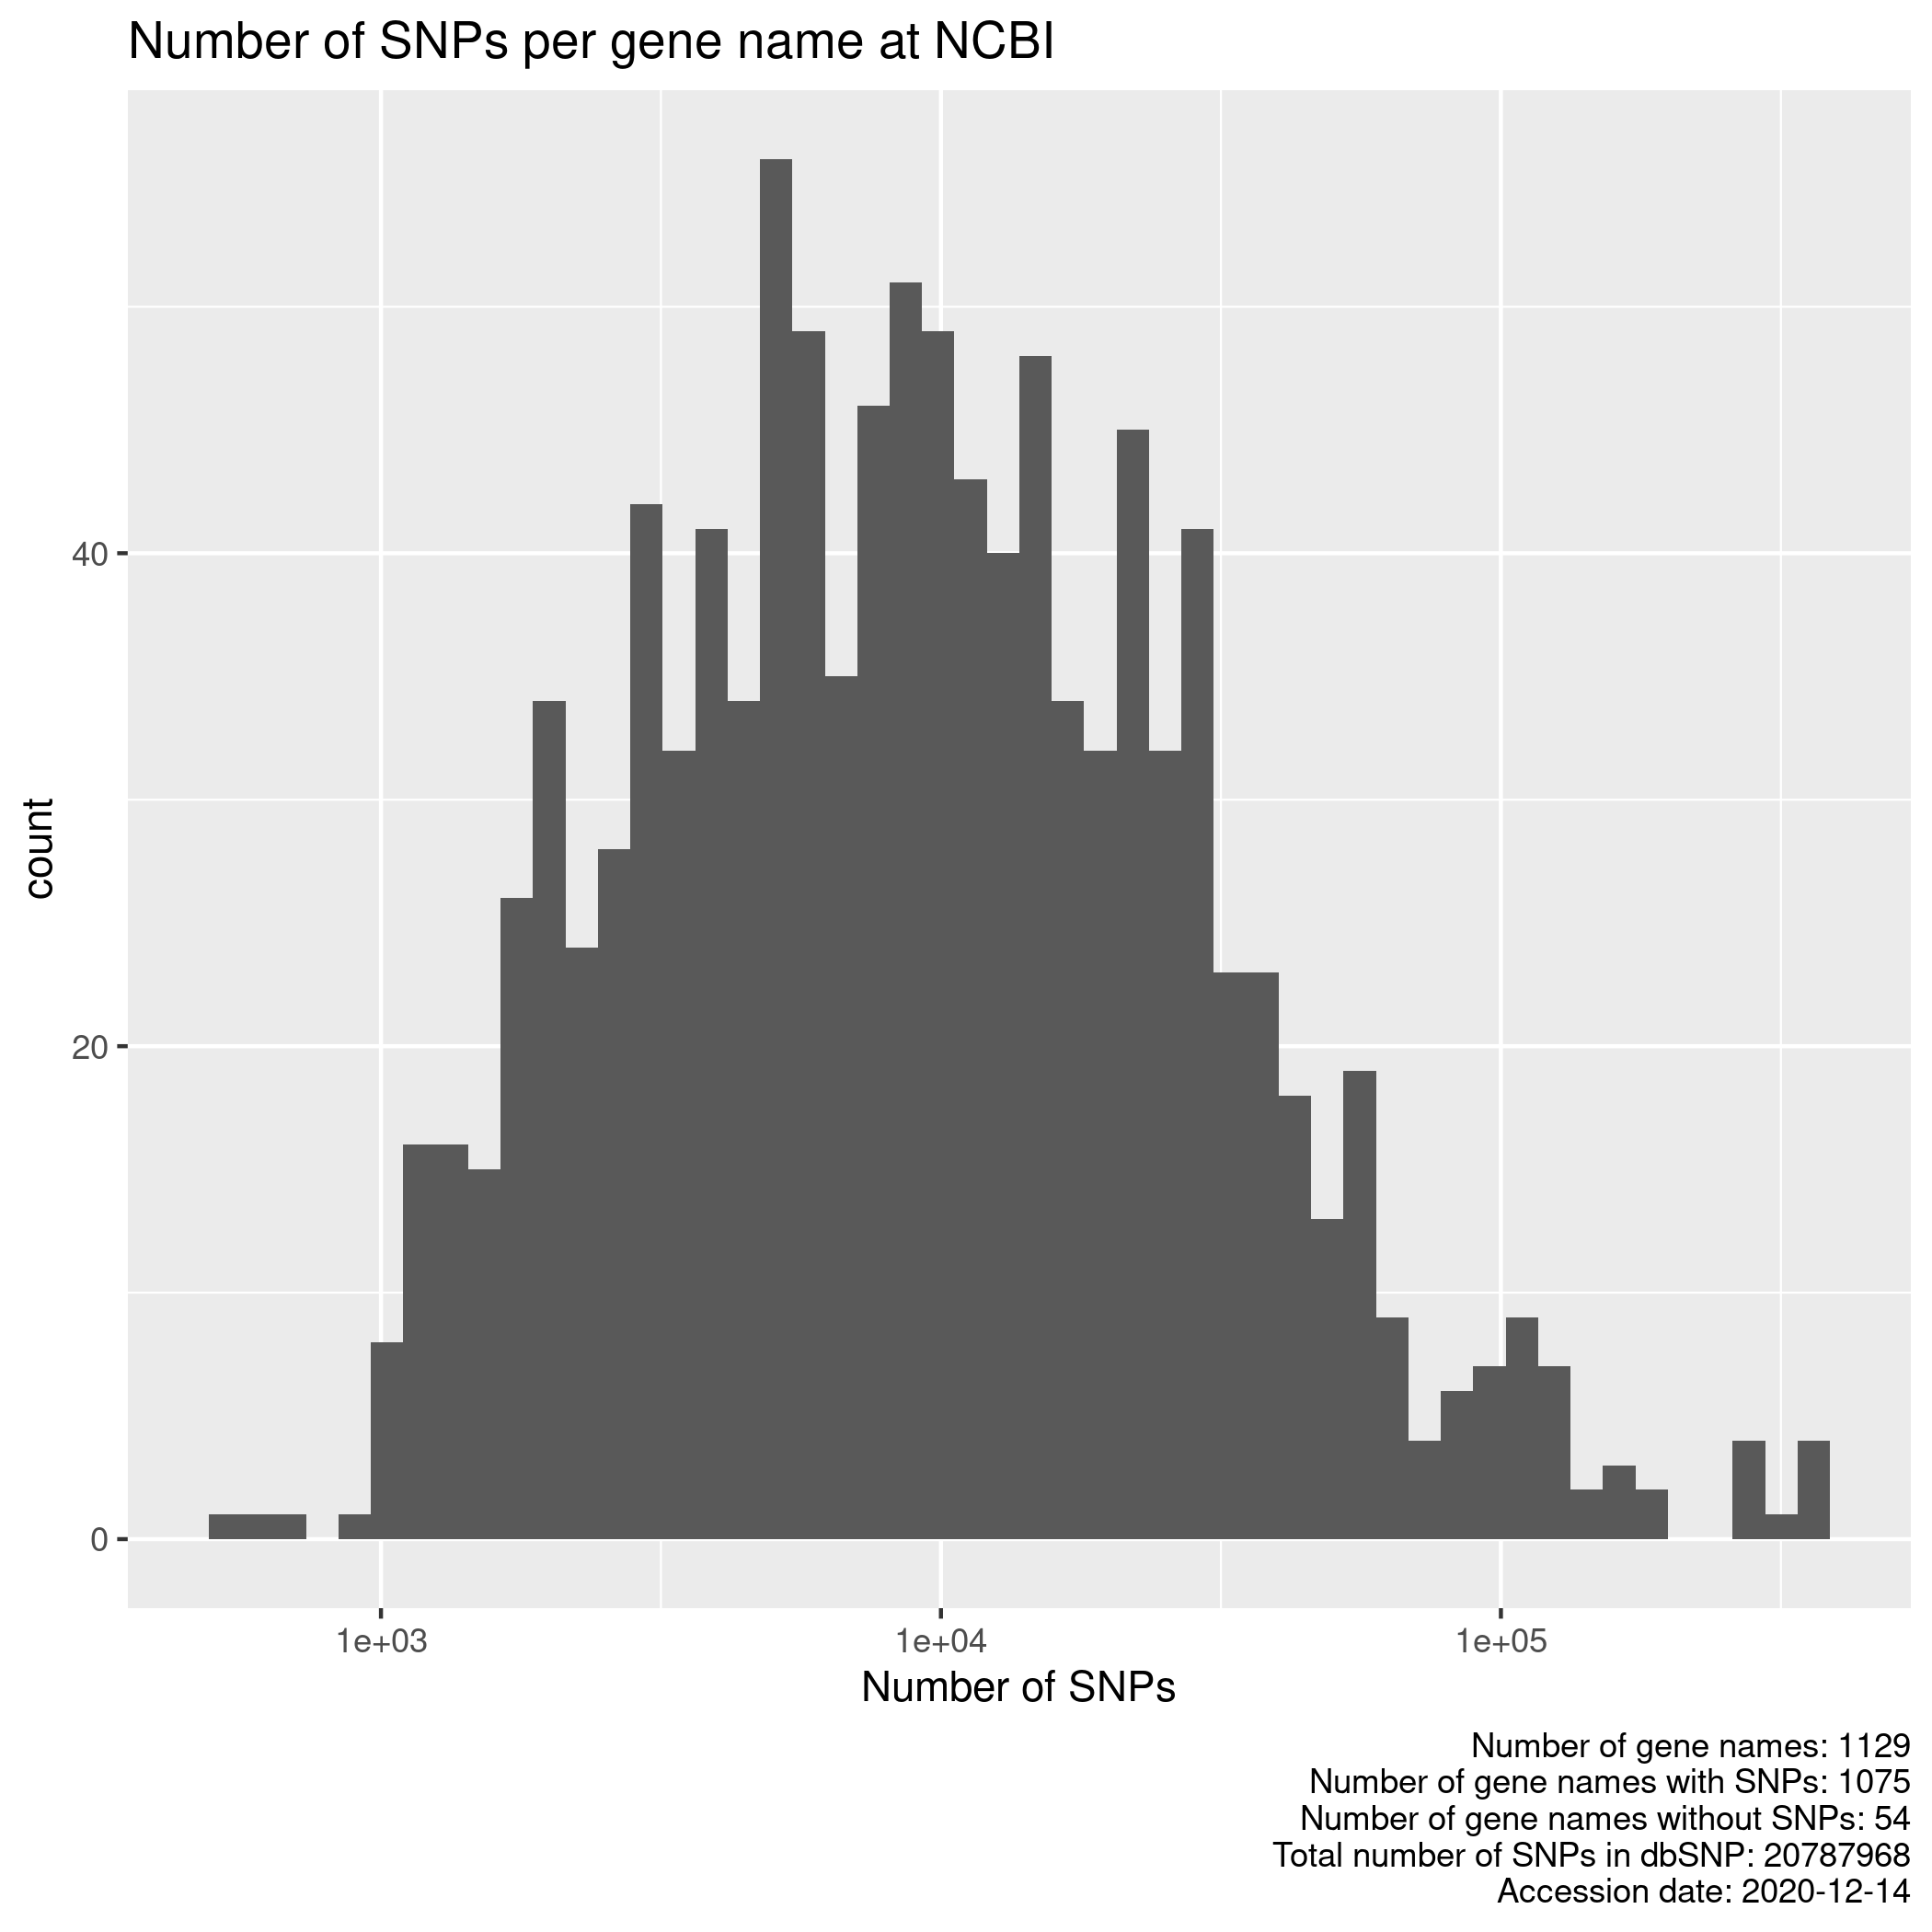
\includegraphics[width=\textwidth]{ncbi_peregrine_results/fig_snps_per_gene_name_ncbi.png}
  \caption{
    Distribution of the number of SNPs per gene name in the NCBI database.
  }
  \label{fig:snps_per_gene_name_ncbi}
\end{figure}

\begin{figure}[!htbp]
  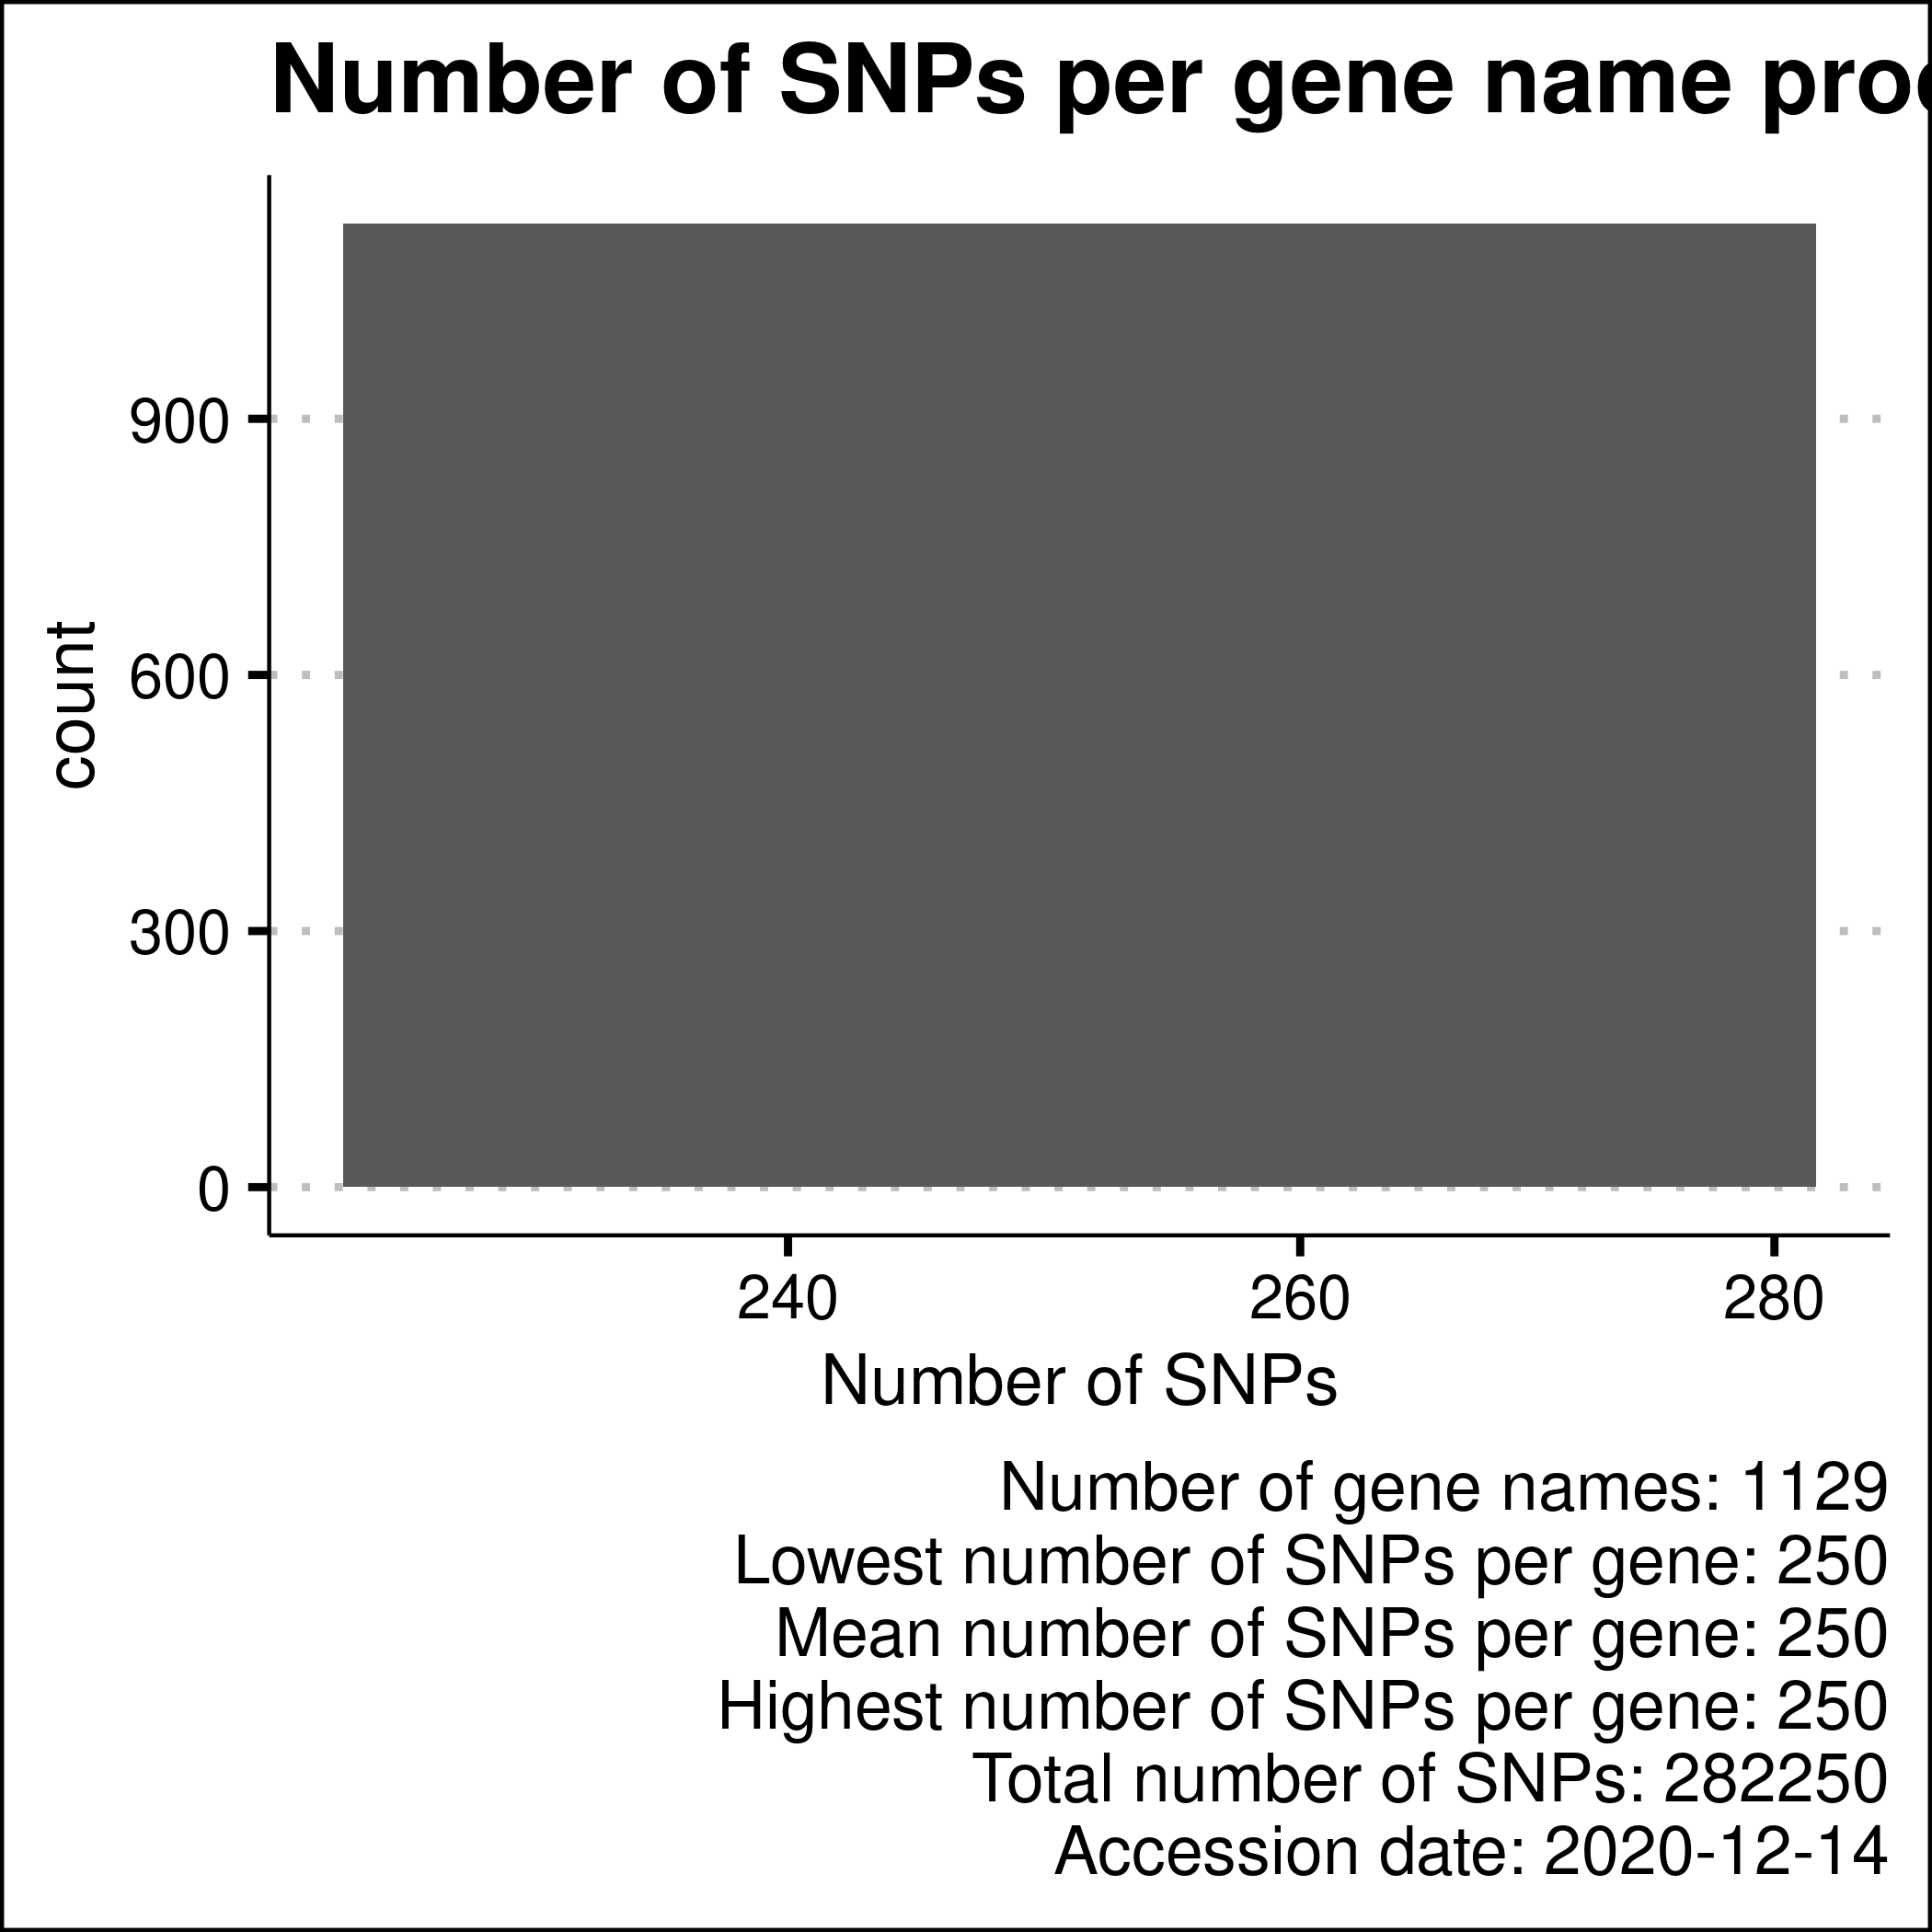
\includegraphics[width=\textwidth]{ncbi_peregrine_results/fig_snps_per_gene_name_processed.png}
  \caption{
    Distribution of the number of protein variations and SNPs per gene name processed.
  }
  \label{fig:snps_per_gene_name_processed}
\end{figure}

\begin{figure}[!htbp]
  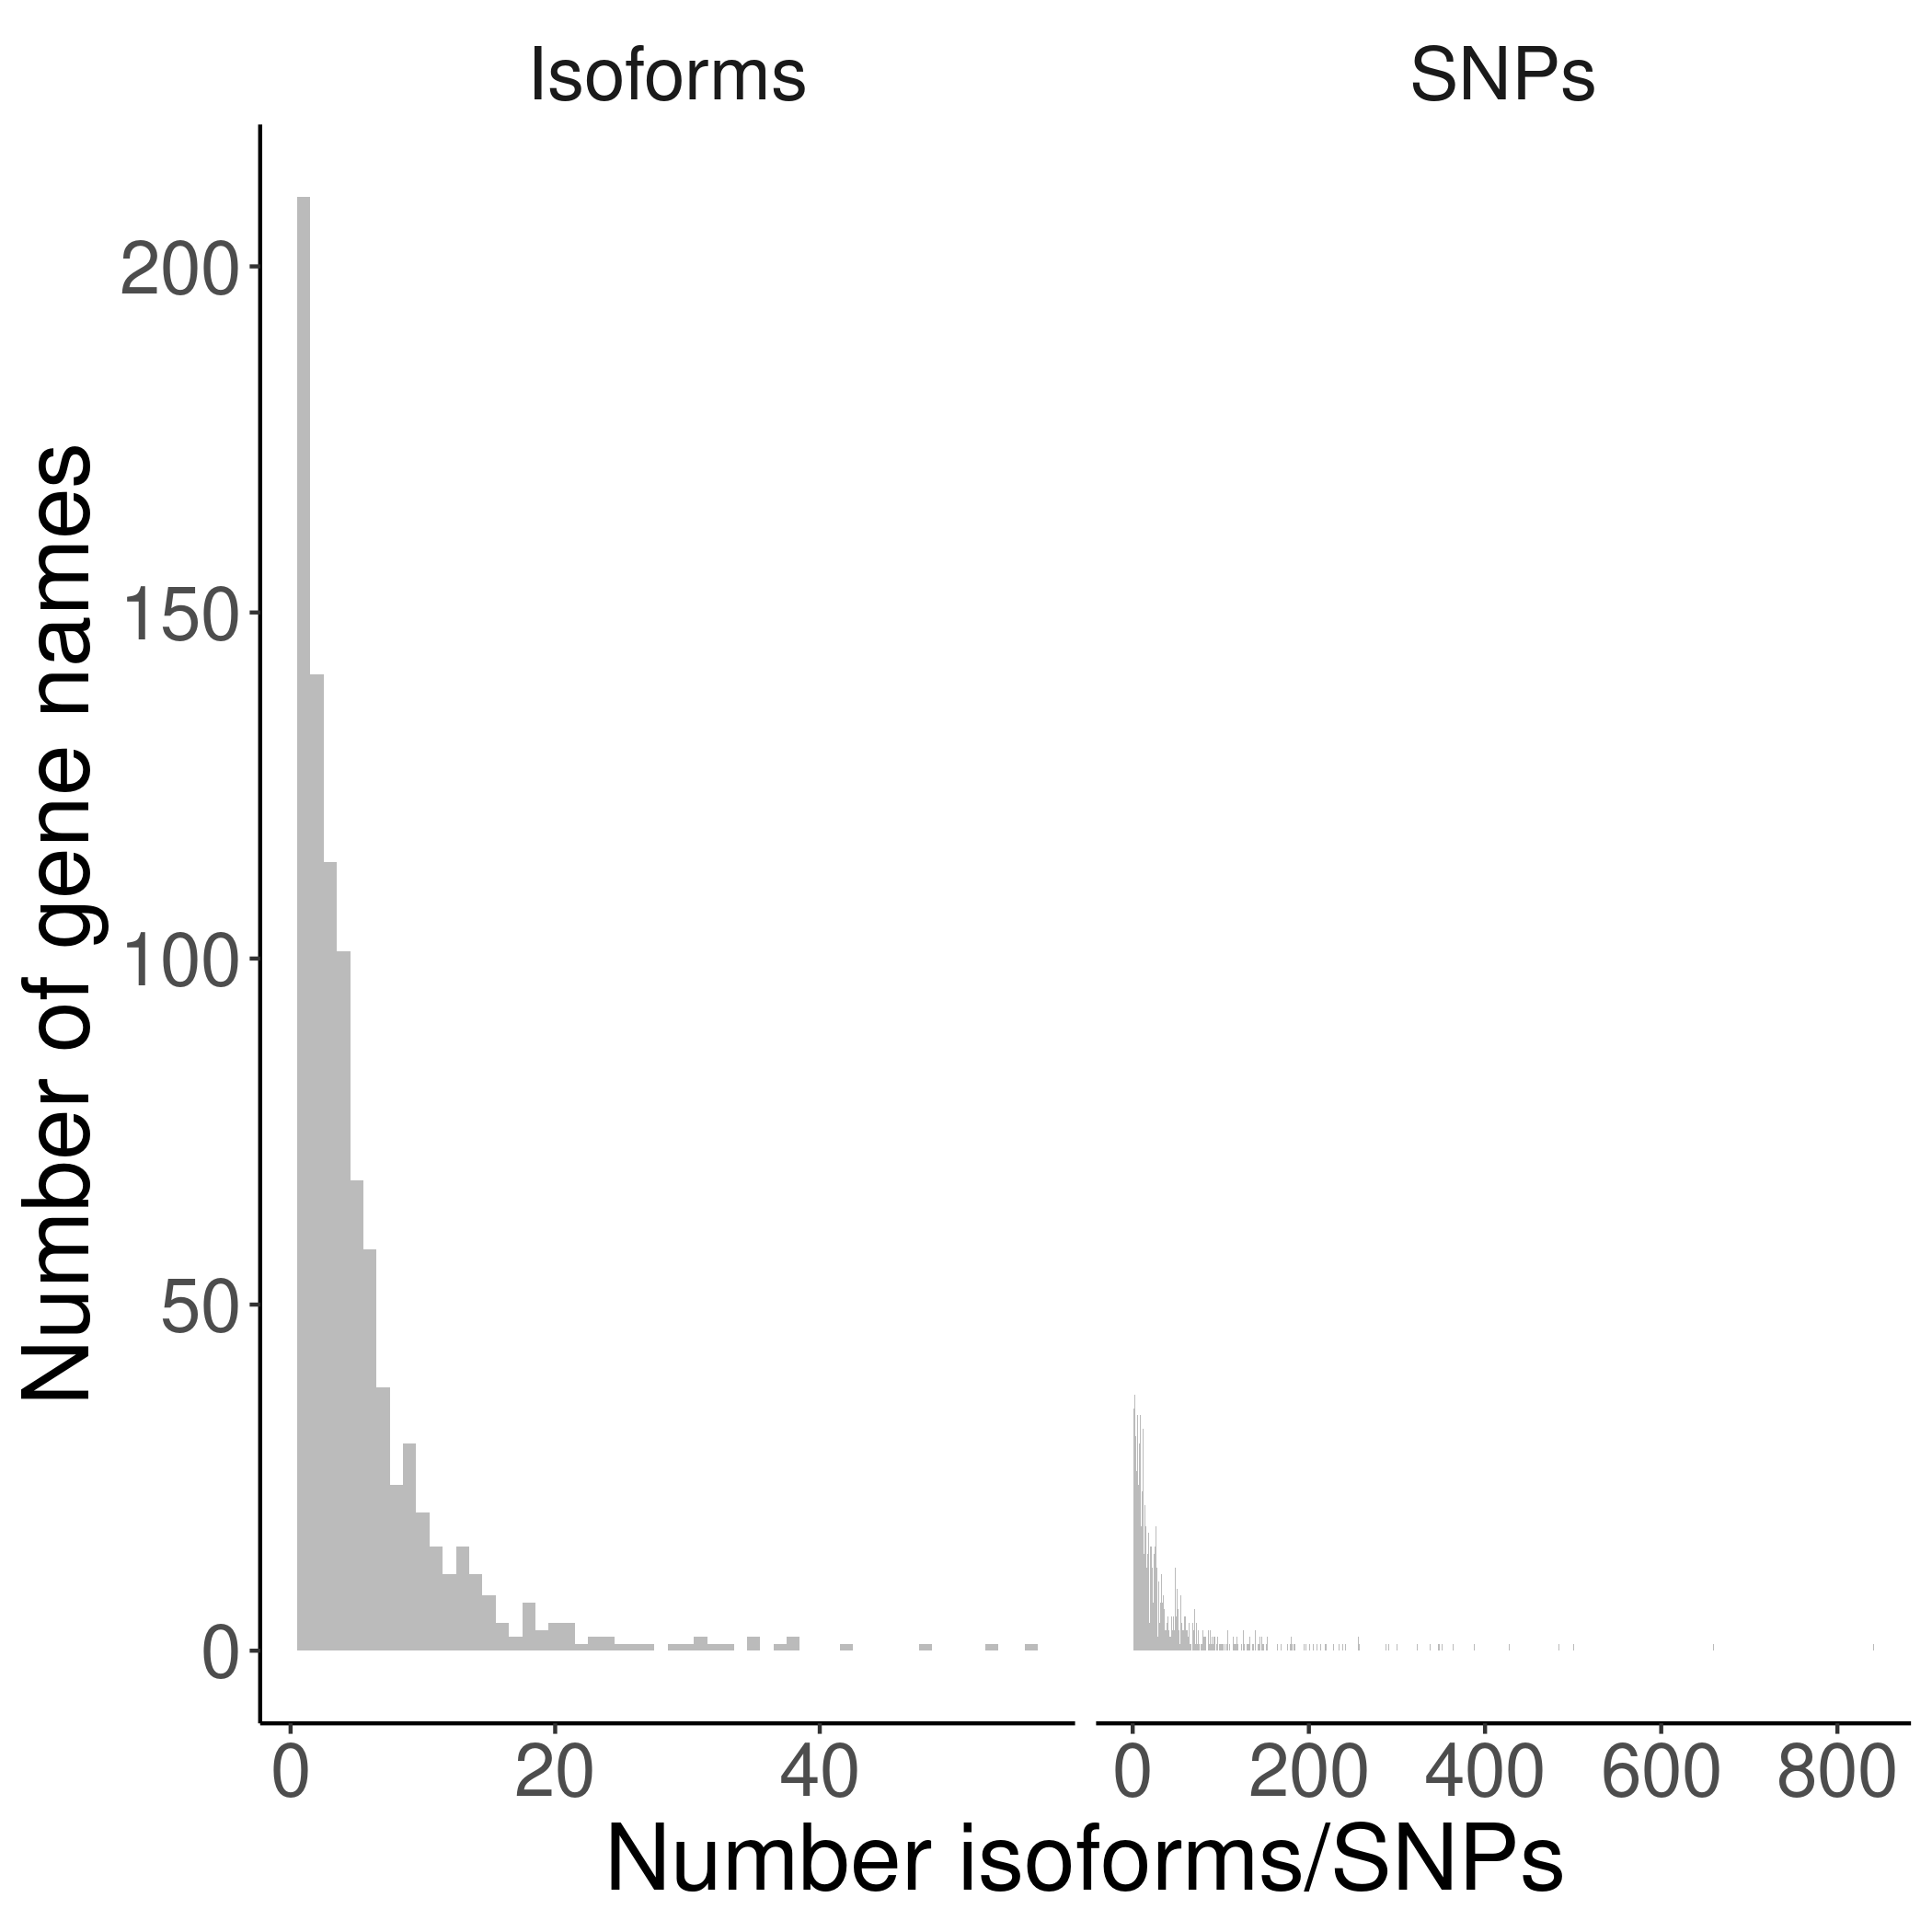
\includegraphics[width=\textwidth]{ncbi_peregrine_results/fig_n_proteins_per_gene_name.png}
  \caption{
    Histogram of the number of proteins found per gene name.
    Most often, a gene name is associated with one protein. 
  }
  \label{fig:n_proteins_per_gene_name}
\end{figure}


\begin{figure}[!htbp]
  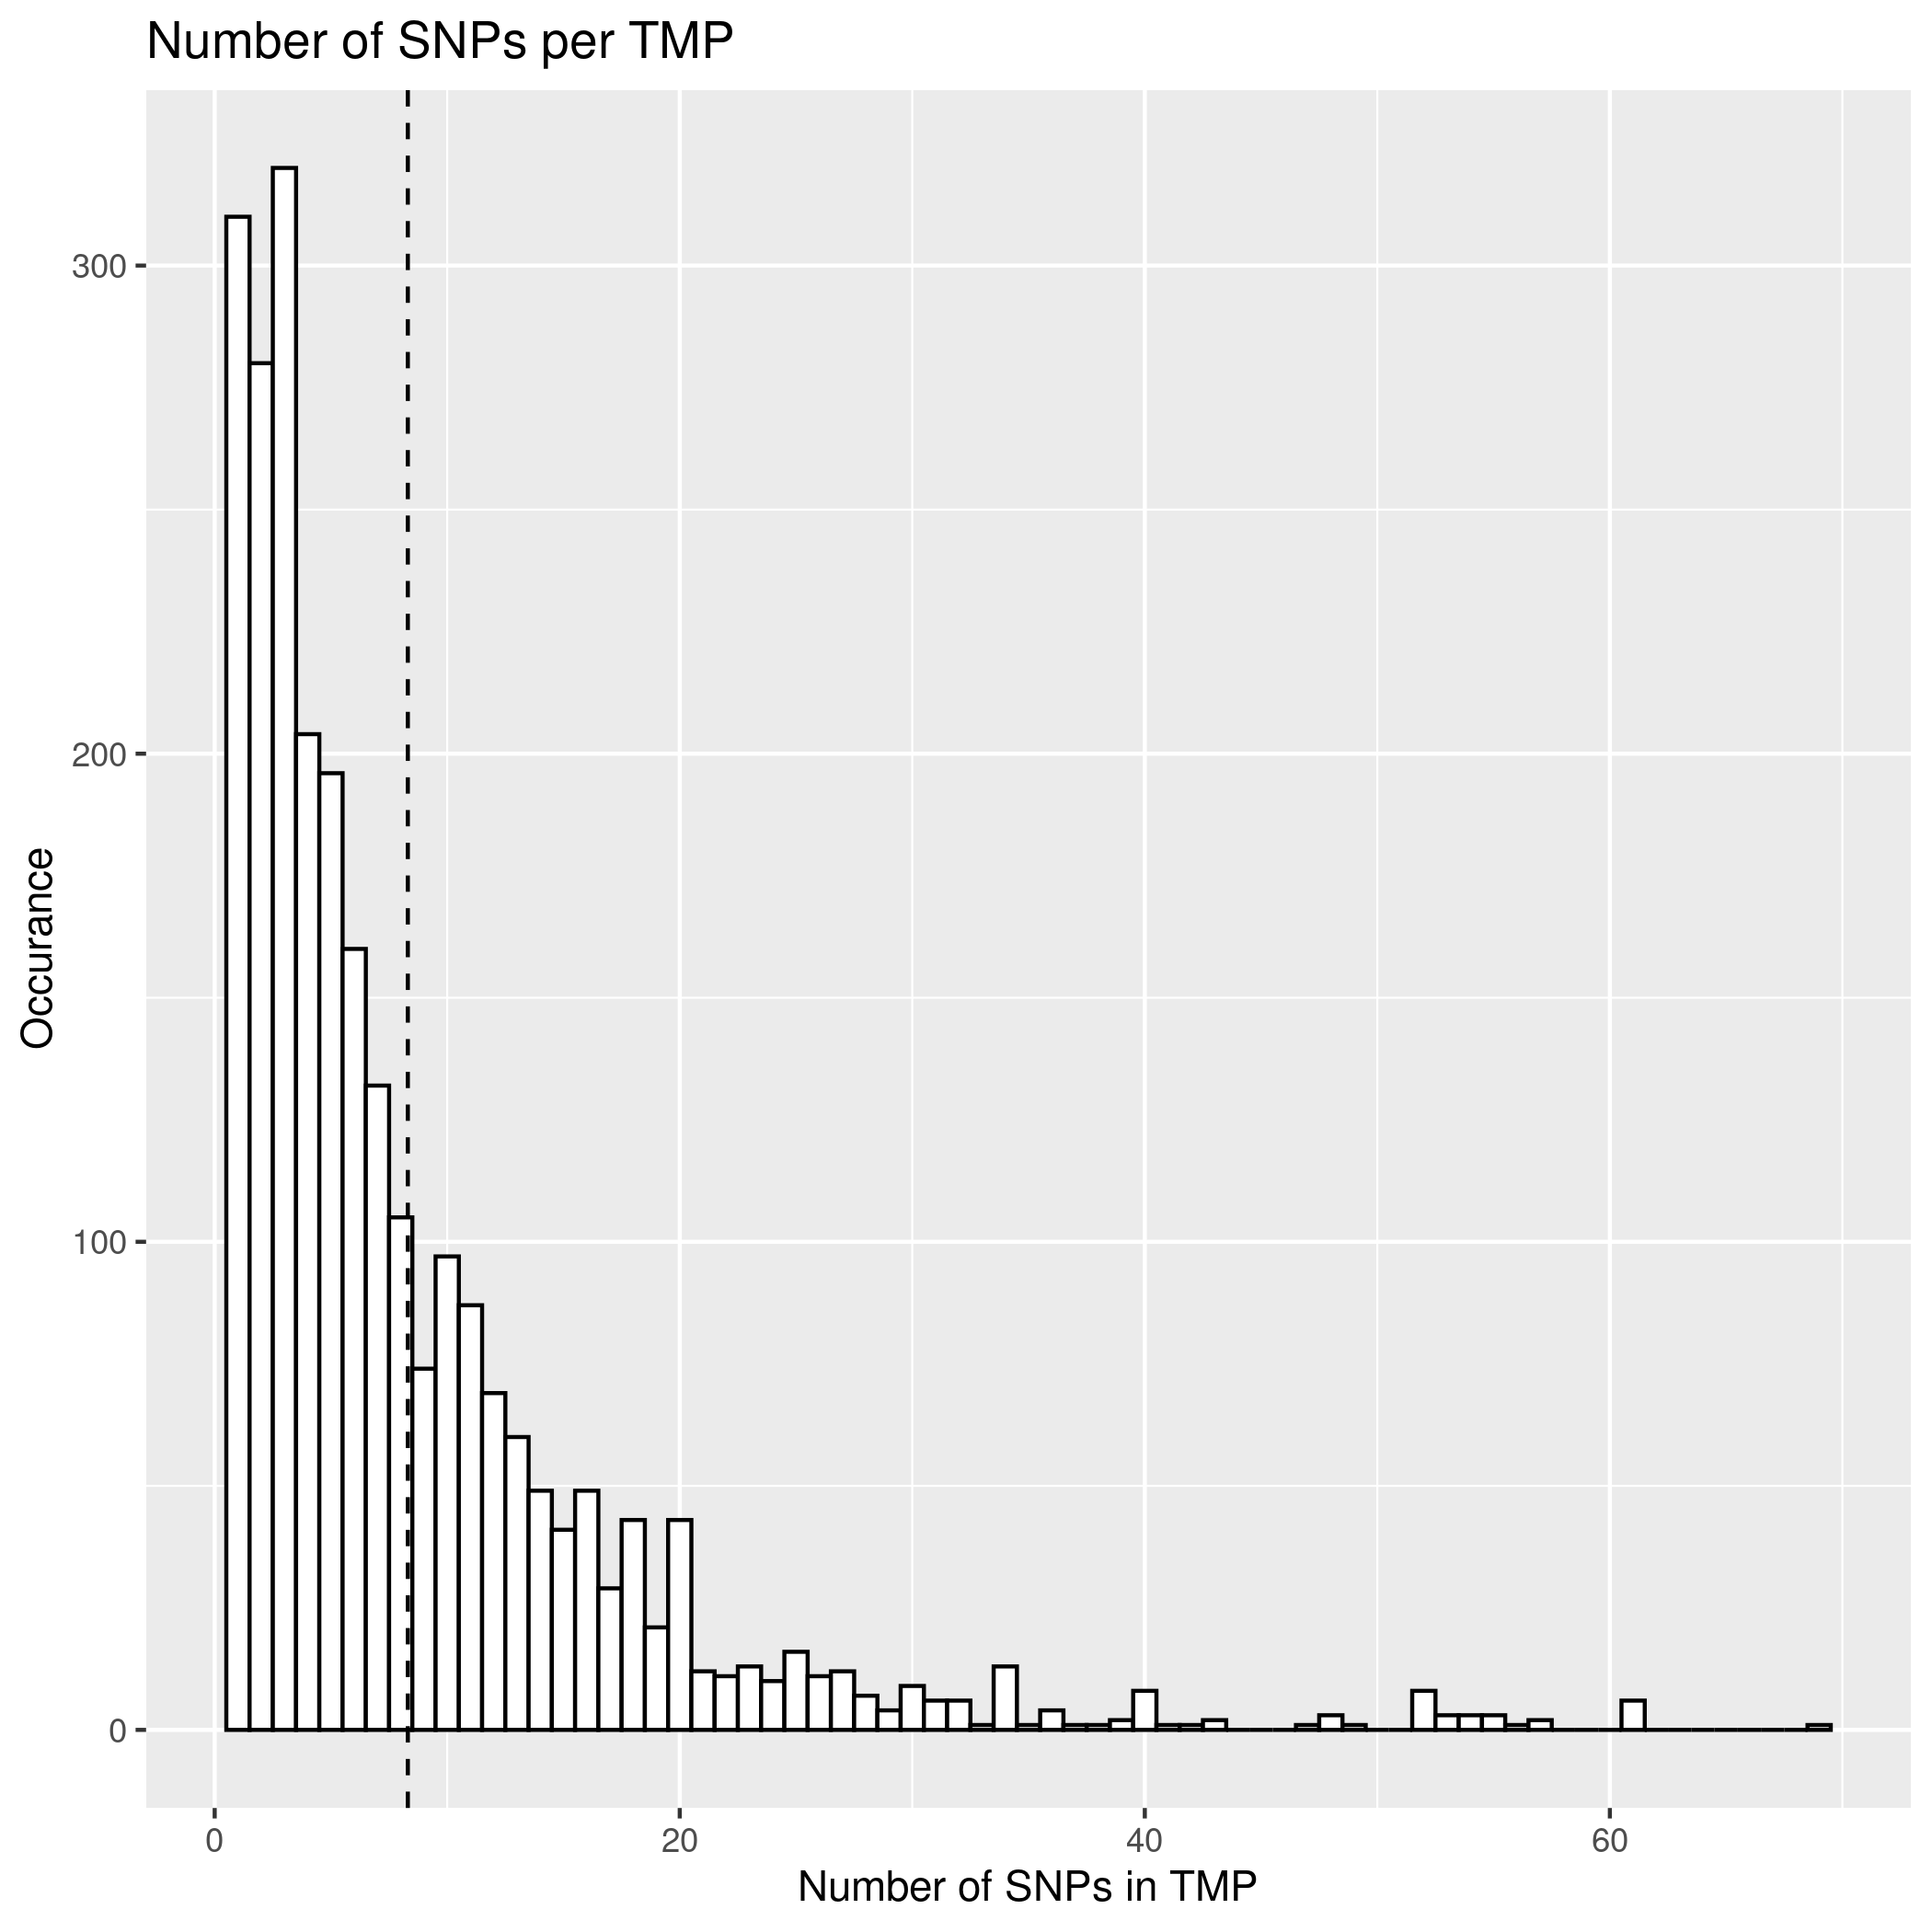
\includegraphics[width=\textwidth]{ncbi_peregrine_results/fig_n_snps_per_tmp.png}
  \caption{
    Histogram of the number of SNPs per trans-membrane protein.
  }
  \label{fig:fig_n_snps_per_tmp}
\end{figure}

\begin{figure}[!htbp]
  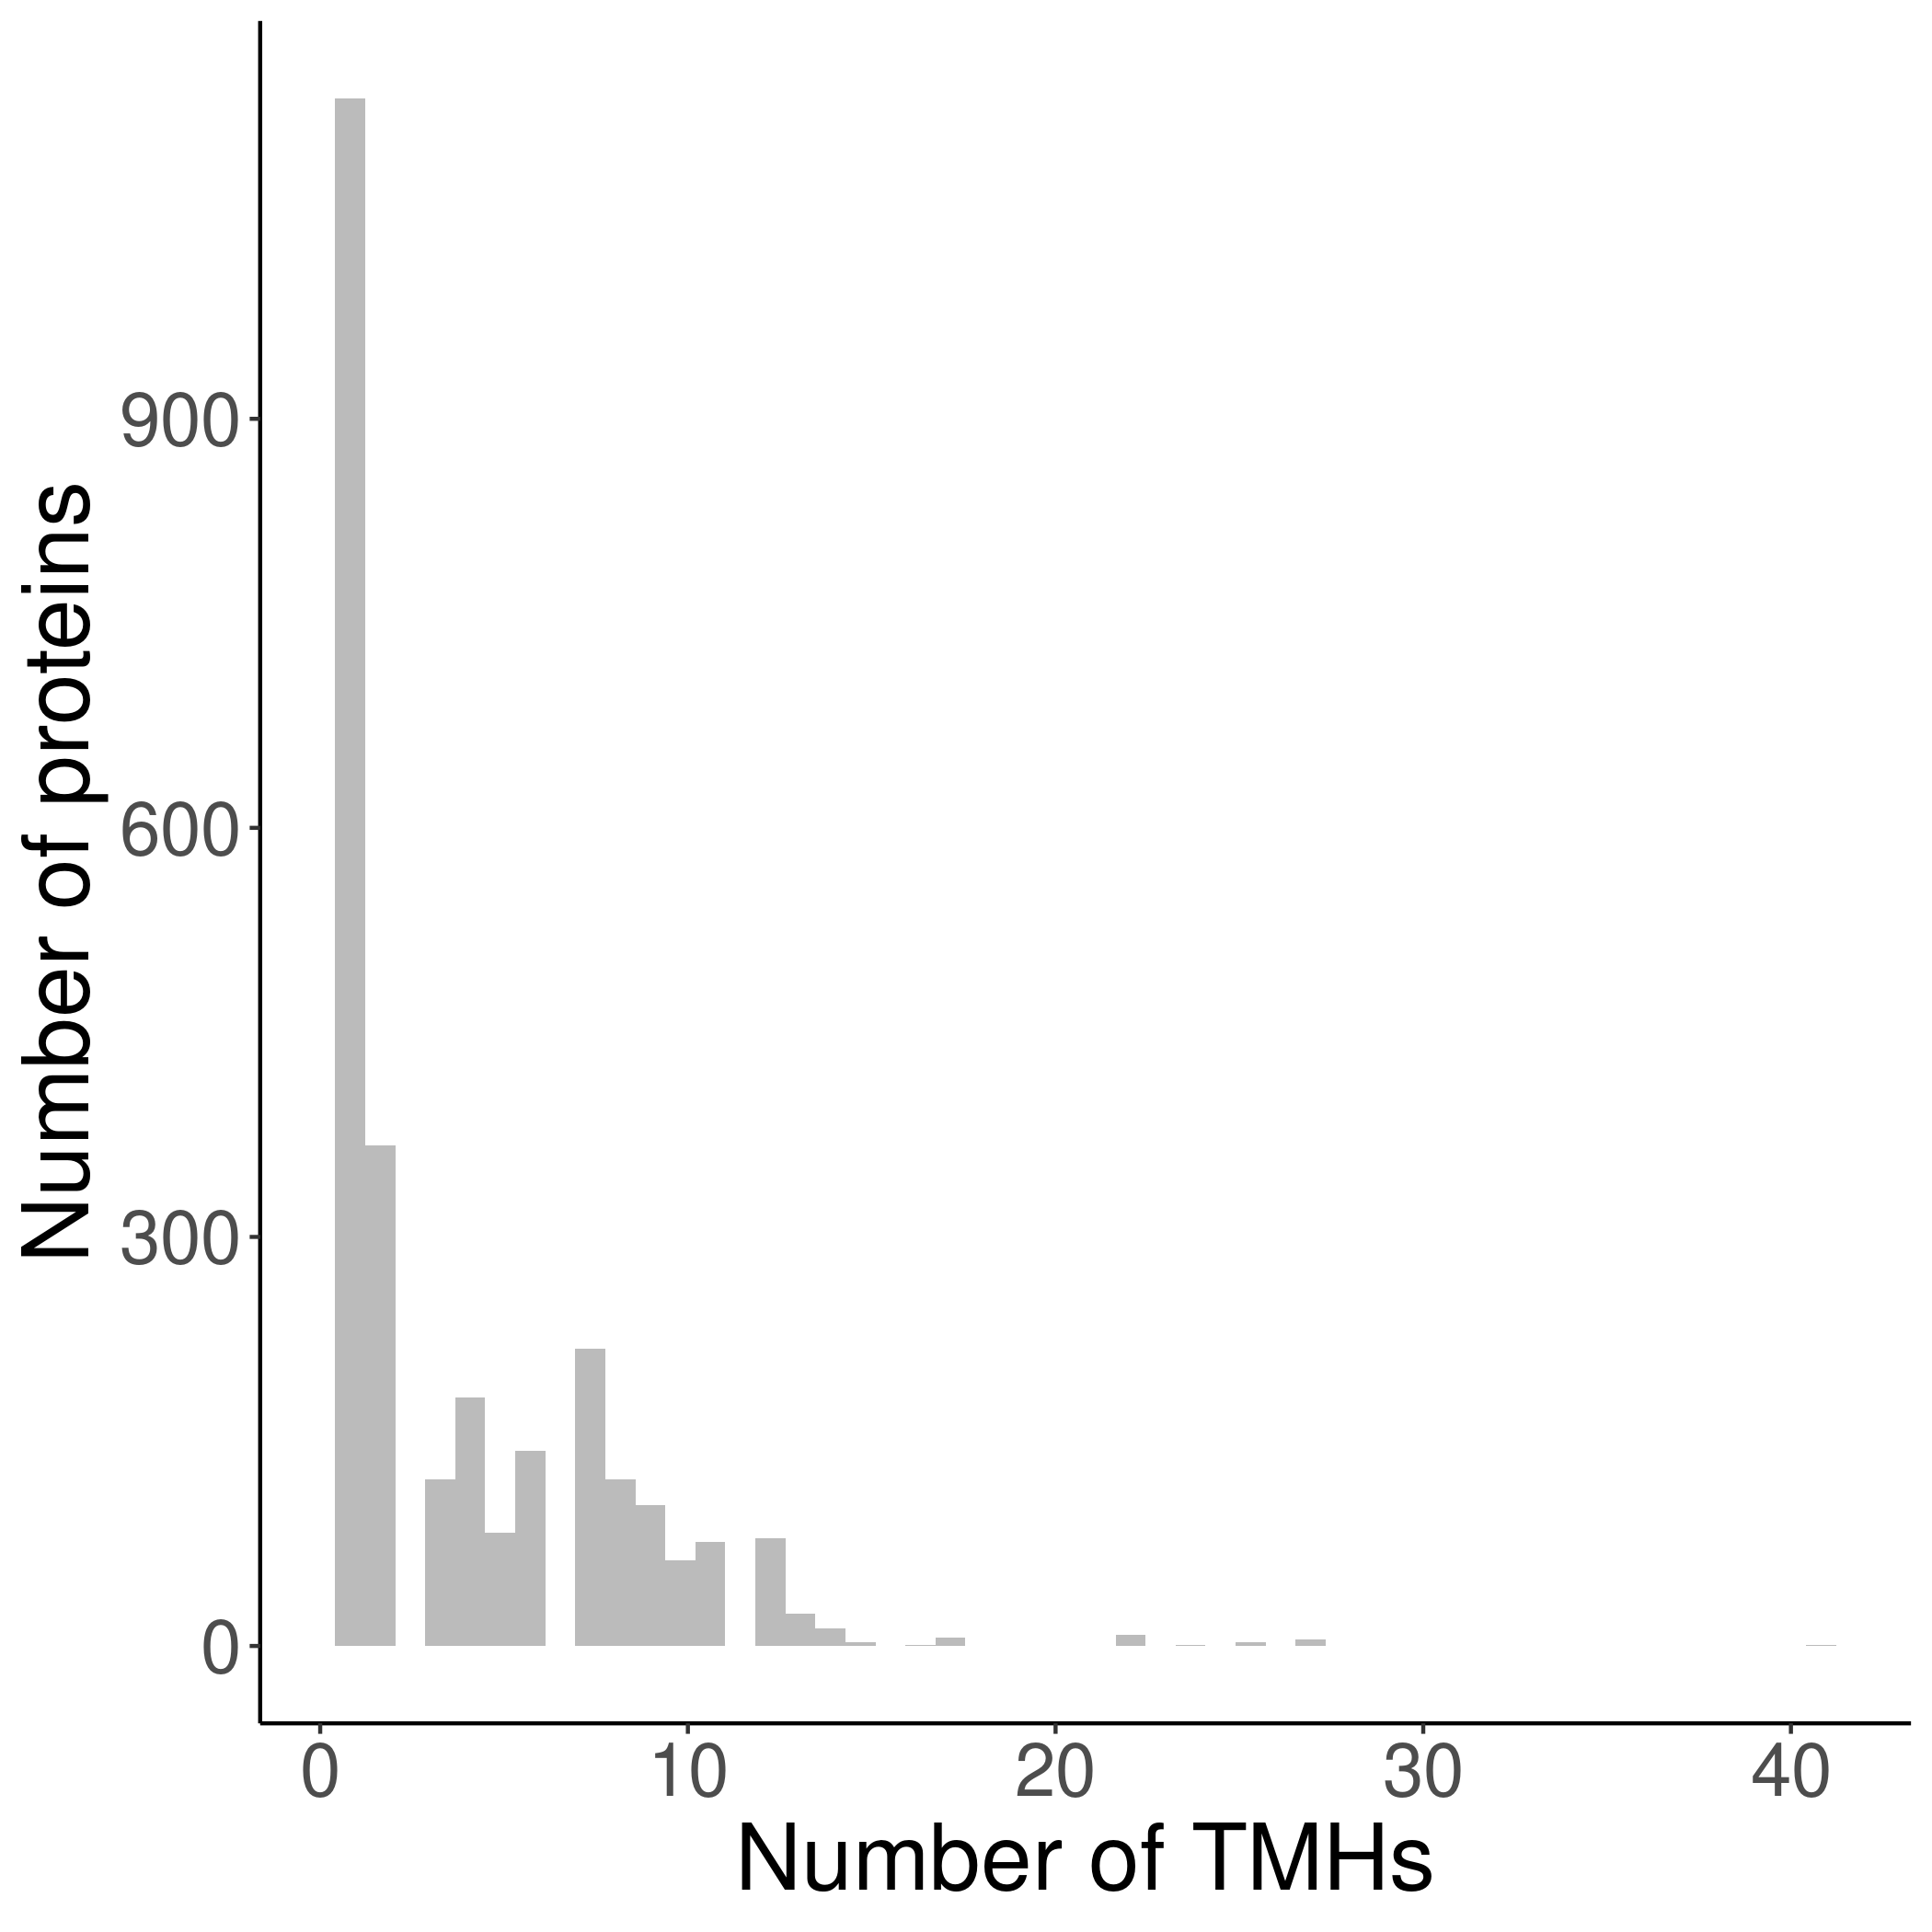
\includegraphics[width=\textwidth]{ncbi_peregrine_results/fig_n_tmhs_per_protein.png}
  \caption{
    Histogram of the number of TMHs predicted per protein,
    for the trans-membrane proteins used.
  }
  \label{fig:fig_n_tmhs_per_protein}
\end{figure}


% \paragraph{Relative position of SNPs}

To verify if SNPs were sampled uniformly
over proteins, we show the distribution 
of the relative position in figure \ref{fig:snp_rel_pos}.
We find no clear evidence of a bias.

% \paragraph{Statistics}

Supplementary Table \ref{tab:snp_stats} shows the statistics for all
SNPs, where supplementary Tables \ref{tab:snp_stats_per_spanner_single}
and \ref{tab:snp_stats_per_spanner_multi} show the
statistics for only single-spanners and multi-spanners respectively.
 
% Label: tab:snp_stats
\begin{table}

\caption{\label{tab:snp_stats}Statistics for the multi-spanners. p = p value. n = number of SNPs. n\_success = number of SNPs found in TMHs (dashed blue line). E(n\_success) = expected number of SNPs to be found in TMHs (dashed red line). }
\centering
\begin{tabular}[t]{l|l}
\hline
parameter & value\\
\hline
p & 6.820823e-11\\
\hline
n & 21208\\
\hline
n\_success & 3803\\
\hline
E(n\_success) & 4140.56\\
\hline
\end{tabular}
\end{table}

% Label: tab:snp_stats_per_spanner_single
\begin{table}

\caption{\label{tab:snp_stats_per_spanner_single}Statistics for the single-spanners. p = p value. n = number of SNPs in single-spanners. n\_success = number of SNPs found in TMHs of single-spanners (dashed blue line). E(n\_success) = expected number of SNPs to be found in TMHs of single-spanners. }
\centering
\begin{tabular}[t]{l|l}
\hline
parameter & value\\
\hline
p & 0.3189532\\
\hline
n & 8186\\
\hline
n\_success & 452\\
\hline
E(n\_success) & 462.1535\\
\hline
\end{tabular}
\end{table}


% Label: tab:snp_stats_per_spanner_multi
\begin{table}

\caption{\label{tab:snp_stats_per_spanner_multi}Statistics for the multi-spanners. p = p value. n = number of SNPs in multi-spanners. n\_success = number of SNPs found in TMHs of multi-spanners (dashed blue line). E(n\_success) = expected number of SNPs to be found in TMHs of multi-spanners  (dashed red line). }
\centering
\begin{tabular}[t]{l|l}
\hline
parameter & value\\
\hline
p & 4.388709e-14\\
\hline
n & 13386\\
\hline
n\_success & 3377\\
\hline
E(n\_success) & 3767.26\\
\hline
\end{tabular}
\end{table}

% Process all floats before going to a next page
\clearpage

%%%%%%%%%%%%%%%%%%%%%%%%%%%%%%%%%%%%%%%%%%%%%%%%%%%%%%%%%%%%%%%%%%%%%%%%%%%%%%%%
\section{Presentation of TMH-derived epitopes when two amino acids overlap}
%%%%%%%%%%%%%%%%%%%%%%%%%%%%%%%%%%%%%%%%%%%%%%%%%%%%%%%%%%%%%%%%%%%%%%%%%%%%%%%%

In our experiment, we define a TMH-derived epitope as a peptide that overlaps
with a TMH for at least one amino acid. 
One could argue that we should use a higher number of overlapping amino acids, so that the epitope has a higher TMH coverage.
We chose not to, for two reason: (1) epitopes that overlap
with a TMH for 1 AA already, cannot be processed by the proteasome in a known and conventional way as it still requires extraction from the membrane
(2) whatever number of overlapping amino acids we use, we expect the pattern to be the same as the chance that an epitope stems from a TMH is equally reduced.
However, using only 1 AA gives the most TMH-derived epitopes and hence the highest statistical
power.

To prove this point, we did exactly the same analysis 
as shown in Figure 1A,
yet with defining a TMH-derived epitope as an epitope that overlaps with a TMH
for at least 2 AAs, as shown in Figure \ref{fig:bbbq_1_smart_results_2aas}.
As these two figures look identical, 
we also added the counts as numbers,
with Table \ref{tab:tmh_binders_mhc2_2aas} showing the same data
as \ref{tab:tmh_binders_mhc2}, except the former uses 2 AAs overlap.
Likewise, Table \ref{tab:tmh_binders_mhc1_2aas} showing the same data
as \ref{tab:tmh_binders_mhc1}, except the former uses 2 AAs overlap.

\begin{figure}[!htbp]
  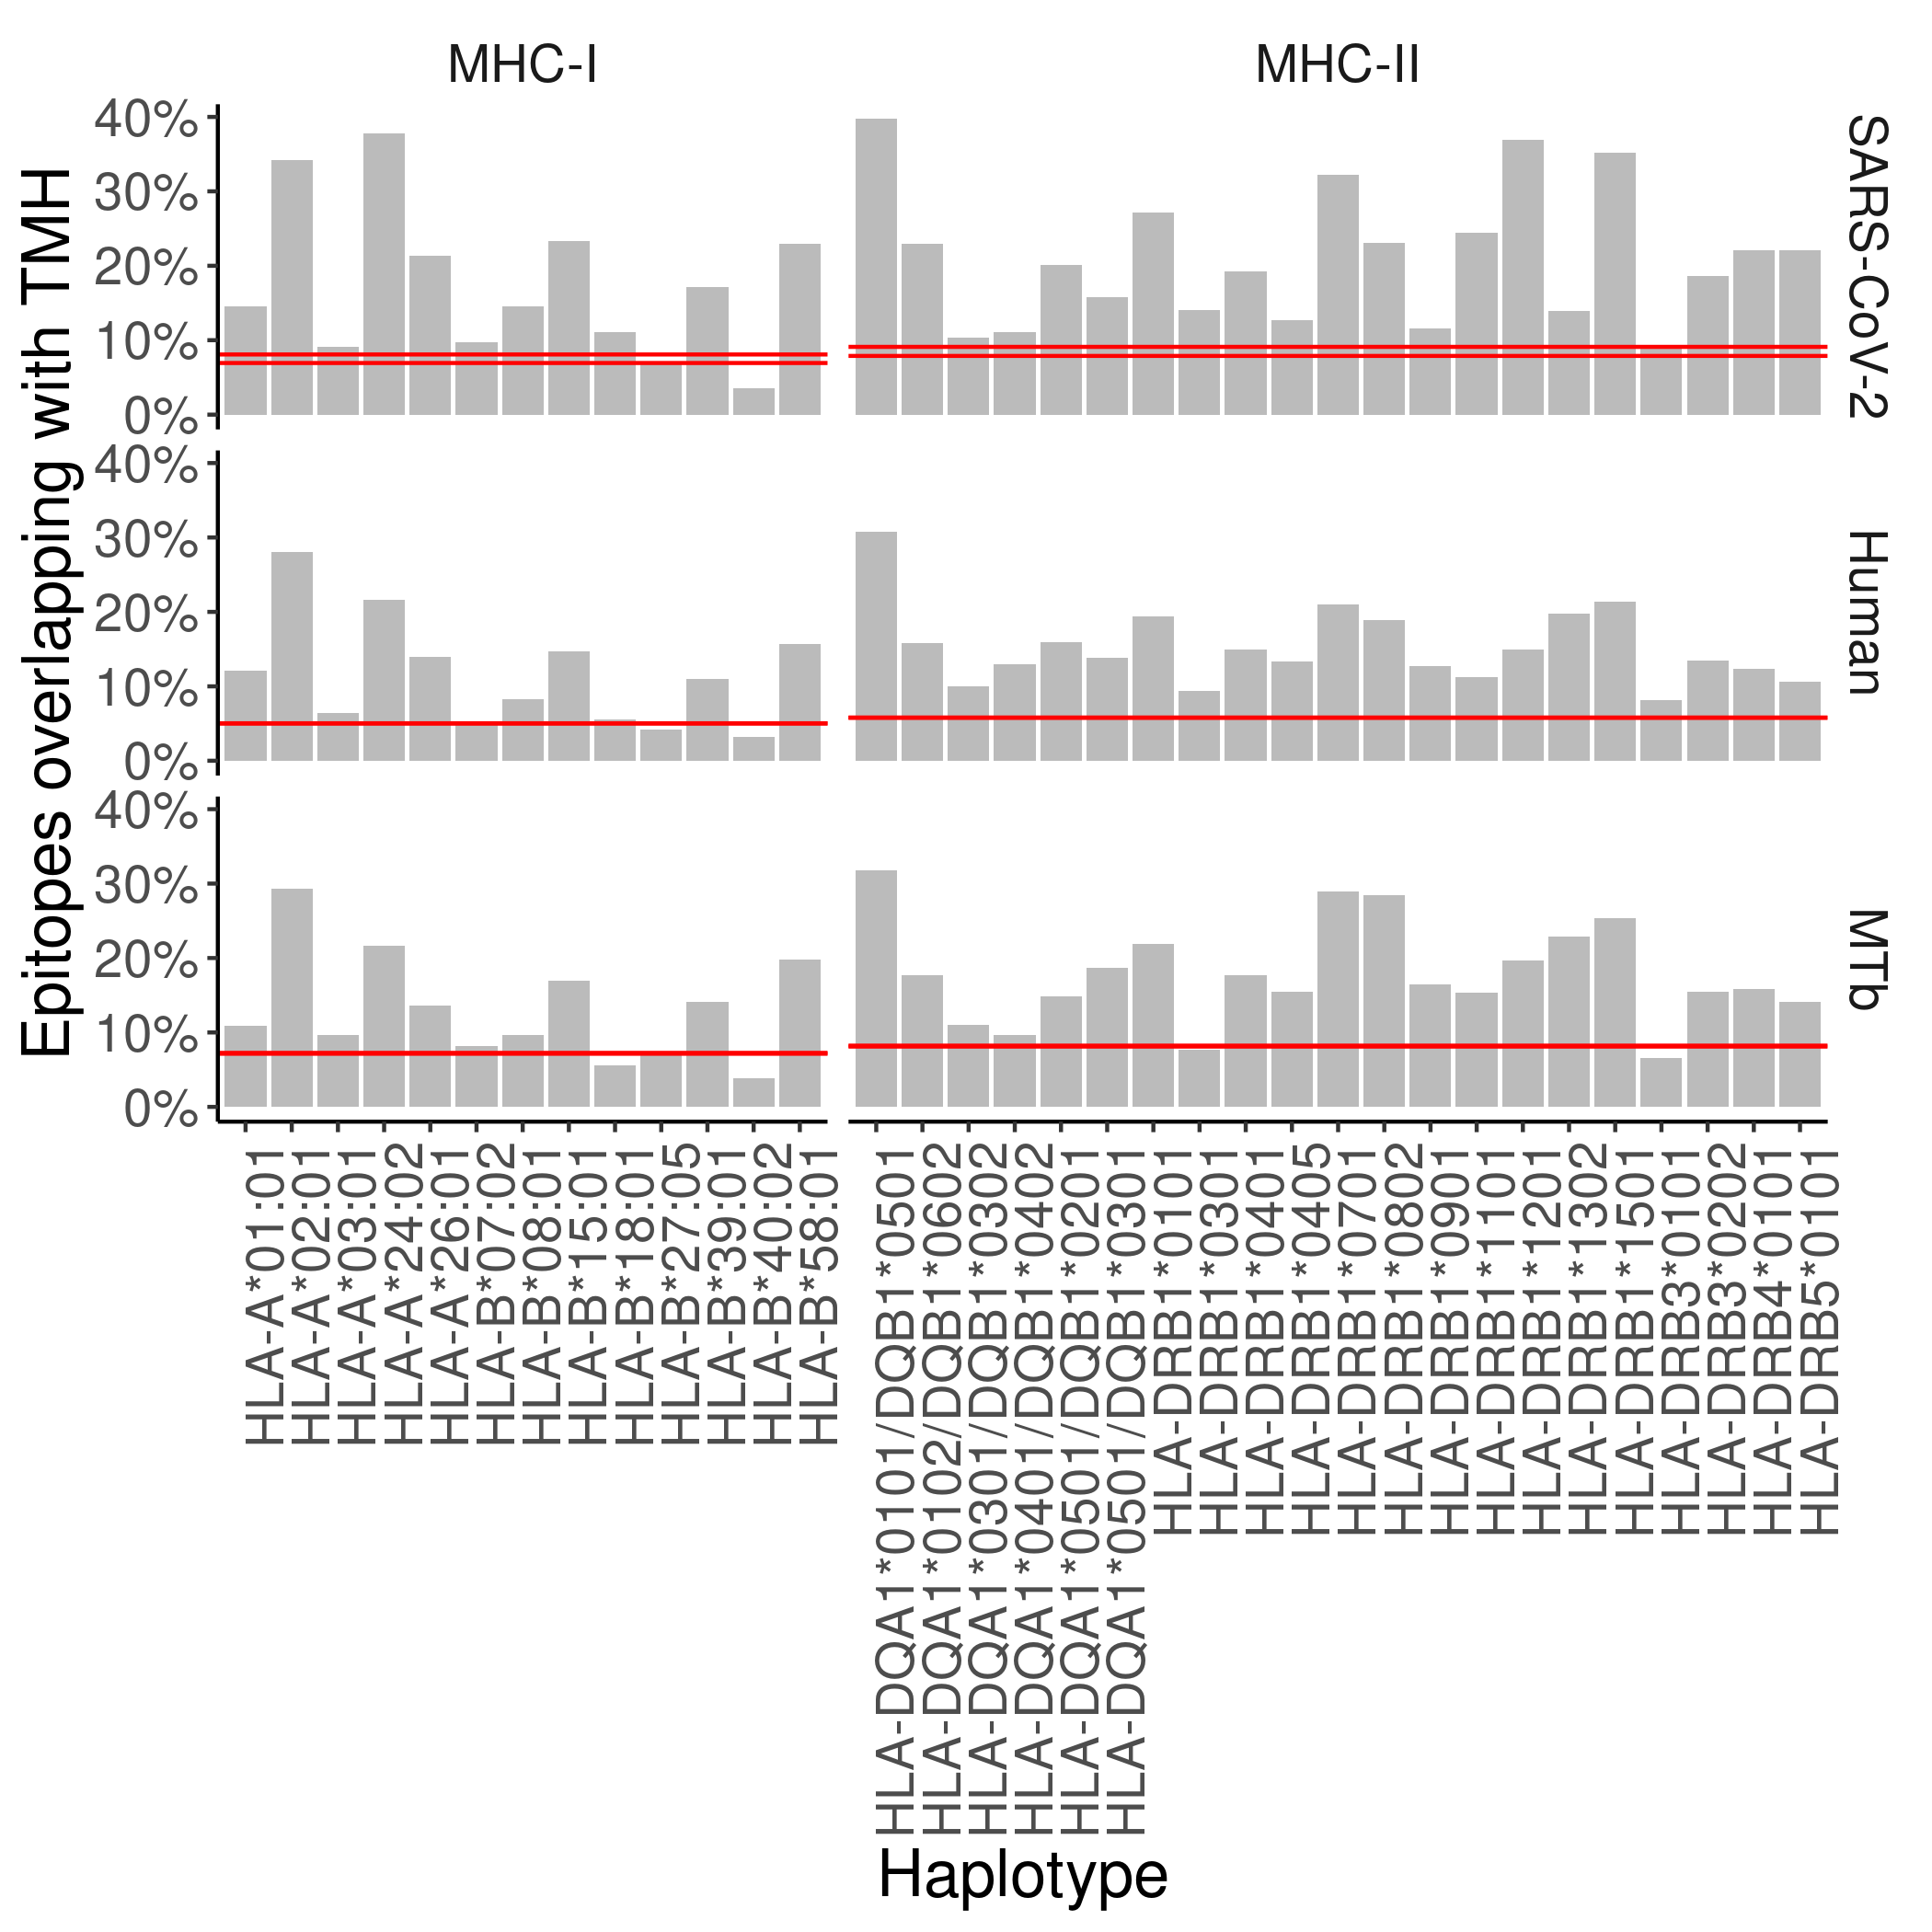
\includegraphics[width=\textwidth]{bbbq_1_smart_2aa_results/fig_f_tmh_2_panel.png}
  \caption{
    The percentage of epitopes for MHC-I and -II alleles that are predicted to 
    overlap with TMHs (for at least two amino acids) 
    for the proteomes of SARS-CoV-2 (top row), human (middle 
    row) and \emph{M. tuberculosis} (bottom row).
    The pair of dashed lines in each plot indicate the lower and upper bound of the 99\% confidence interval.
    See supplementary Tables \ref{tab:tmh_binders_mhc2_2aas} and \ref{tab:tmh_binders_mhc1_2aas}
    for the exact TMH and  epitope counts.
  }
  \label{fig:bbbq_1_smart_results_2aas}
\end{figure}

% Label: tab:tmh_binders_mhc2_2aas
\input{bbbq_1_smart_2aa_results/table_tmh_binders_mhc2_2.latex}

% Label: tab:tmh_binders_mhc1_2aas
\input{bbbq_1_smart_2aa_results/table_tmh_binders_mhc1_2.latex}

%%%%%%%%%%%%%%%%%%%%%%%%%%%%%%%%%%%%%%%%%%%%%%%%%%%%%%%%%%%%%%%%%%%%%%%%%%%%%%%%
\section*{Abbreviations}
%%%%%%%%%%%%%%%%%%%%%%%%%%%%%%%%%%%%%%%%%%%%%%%%%%%%%%%%%%%%%%%%%%%%%%%%%%%%%%%%

\begin{table}[h]
  \begin{tabular}{ll}
    Abbreviation & Full               \\ 
    \hline
ER & Endoplasmatic reticulum \\
ERAD & ER-associated degradation \\
HLA & Human leukocyte antigen \\
IEDB & Immune Epitope Database  \\
LB & lipid body \\
MAP & Membrane-associated protein \\
MHC & Major histocompatibility complex \\
MVB & Multivesicular body \\
PLC & Peptide-loading complex \\
SNP & Single nucleotide polymorphism \\
TMH & Transmembrane helix         \\
    TMP & Transmembrane protein
  \end{tabular}
\end{table}


%%%%%%%%%%%%%%%%%%%%%%%%%%%%%%%%%%%%%%%%%%%%%%%%%%%%%%%%%%%%%%%%%%%%%%%%%%%%%%%%
\bibliographystyle{frontiersinSCNS_ENG_HUMS} % for Science, Engineering and Humanities and Social Sciences articles, for Humanities and Social Sciences articles please include page numbers in the in-text citations
%\bibliographystyle{frontiersinHLTH&FPHY} % for Health, Physics and Mathematics articles
\bibliography{bbbq_article}


\end{document}
